% ---------------------------------------------------------------------------
% main.tex — MONOGRAFIA — Laboratório 404
% Autor: William da Silva Vianna — Instituto Federal Fluminense
% Compilação: pdflatex -> bibtex -> pdflatex -> pdflatex  (ver build.sh)
% Formatação ABNT aplicada manualmente (memoir); modelo institucional a validar.
% ---------------------------------------------------------------------------
\documentclass[12pt,a4paper,oneside]{memoir}

\usepackage[utf8]{inputenc}
\usepackage[T1]{fontenc}
\usepackage[brazil]{babel}
\shorthandoff{"}

\usepackage{lmodern}
\usepackage{microtype}
\usepackage{graphicx}
\graphicspath{{figures/}}
\usepackage{booktabs}
\usepackage{array}
\usepackage{float}
\usepackage{amsmath}
\usepackage{amssymb}
\usepackage{tikz}
\usetikzlibrary{arrows.meta,positioning,shapes.geometric,fit}
\usepackage{pgfplots}
\pgfplotsset{compat=1.18}
\usepackage[hidelinks]{hyperref}
\hypersetup{
  pdftitle={Laboratório 404: desenvolvimento de um jogo sério 3D com inteligência artificial local para apoio ao ensino de automação industrial},
  pdfauthor={William da Silva Vianna},
  pdfsubject={Monografia de graduação em Engenharia},
  pdfkeywords={jogos sérios; automação industrial; grandes modelos de linguagem; inferência local; Godot; Blender}
}

% --- layout ABNT (manual): margens 3/2 cm e espaçamento 1,5 ---
\setlrmarginsandblock{3cm}{2cm}{*}
\setulmarginsandblock{3cm}{2cm}{*}
\checkandfixthelayout
\OnehalfSpacing
\setlength{\parindent}{1.25cm}
\setlength{\parskip}{0pt}
\emergencystretch=1em

% --- capítulos numerados como "1 Título" (sem a palavra Capítulo) ---
\renewcommand{\printchaptername}{\chapnamefont\thechapter}
\renewcommand{\printchapternum}{}

% --- legendas discretas (ABNT) ---
\captionnamefont{\small\bfseries}
\captiontitlefont{\small}

% --- Quadros (float novo + lista própria) ---
\newfloat{quadro}{htbp}{loq}
\floatname{quadro}{Quadro}

% --- abreviações auxiliares ---
\newcommand{\poc}[1]{POC~#1}
\newcommand{\aria}{ARIA}

\begin{document}

% pretextual.tex — elementos pré-textuais (capa, folha de rosto, resumos, listas, sumário)
% Dados fornecidos pelo autor em 2026-09-10: campus, cidade e orientação.
% [VALIDAR COM O AUTOR]: curso exato, banca e demais elementos institucionais.

\frontmatter

% ---------------------------------------------------------------------------
% Capa
% ---------------------------------------------------------------------------
\begin{center}
  \textbf{INSTITUTO FEDERAL FLUMINENSE}\\[2pt]
  Campus: Meu laboratório pessoal\\
  Curso de Engenharia de Controle e Automação [VALIDAR COM O AUTOR]
\end{center}

\vspace{2.5cm}

\begin{center}
  \textbf{WILLIAM DA SILVA VIANNA}
\end{center}

\vspace{3.0cm}

\begin{center}
  \textbf{LABORATÓRIO 404: DESENVOLVIMENTO DE UM JOGO SÉRIO 3D COM\\
  INTELIGÊNCIA ARTIFICIAL LOCAL PARA APOIO AO\\ ENSINO DE AUTOMAÇÃO INDUSTRIAL}
\end{center}

\vfill

\begin{center}
  Campos dos Goytacazes\\
  2026
\end{center}

\newpage

% ---------------------------------------------------------------------------
% Folha de rosto
% ---------------------------------------------------------------------------
\begin{center}
  \textbf{WILLIAM DA SILVA VIANNA}
\end{center}

\vspace{2.5cm}

\begin{center}
  \textbf{LABORATÓRIO 404: DESENVOLVIMENTO DE UM JOGO SÉRIO 3D COM\\
  INTELIGÊNCIA ARTIFICIAL LOCAL PARA APOIO AO\\ ENSINO DE AUTOMAÇÃO INDUSTRIAL}
\end{center}

\vspace{2.5cm}

\hfill
\begin{minipage}{8cm}
  \SingleSpacing
  \footnotesize
  Monografia apresentada ao curso de Engenharia de Controle e Automação
  [VALIDAR COM O AUTOR] do Instituto Federal Fluminense, como requisito
  parcial para obtenção do título de bacharel.\\
  Orientador: o próprio autor.\\
  Área de concentração: automação industrial e tecnologia educacional.
\end{minipage}

\vfill

\begin{center}
  Campos dos Goytacazes\\
  2026
\end{center}

\newpage

% ---------------------------------------------------------------------------
% Resumo
% ---------------------------------------------------------------------------
\chapter*{Resumo}
\addcontentsline{toc}{chapter}{Resumo}

\SingleSpacing

Este trabalho descreve o projeto, o desenvolvimento e a validação técnica do
Laboratório 404, um jogo sério 3D educacional/ficcional no qual uma
inteligência artificial local --- a personagem \aria{} --- participa do mundo
por meio de diálogo, sem nunca controlar o jogo. O problema abordado é
triplo: integrar um grande modelo de linguagem (LLM) a um jogo 3D mantendo
segurança e previsibilidade; executar essa integração em um computador pessoal
sem GPU dedicada; e conduzir o desenvolvimento de forma rastreável, com
requisitos verificáveis e evidências reproduzíveis. A solução foi construída em
seis provas de conceito incrementais (\poc{1} a \poc{6}) sobre o motor Godot~4.5,
com assets 3D modelados no Blender~5.2.1 e um adaptador local em Python/FastAPI
que media a conversa com o Ollama, restringindo a saída do modelo a cinco
intenções validadas em duas camadas independentes, com resposta de
\emph{fallback} obrigatória. A validação combinou uma especificação com
requisitos funcionais e não funcionais, critérios de aceitação no formato
DADO/QUANDO/ENTÃO, uma suíte automatizada \emph{headless} e evidências visuais
geradas por um arnês de captura. Os resultados obtidos na máquina de referência
(AMD Ryzen~7 5700U, GPU integrada) foram: 211 verificações do motor e 16 testes
do adaptador aprovados; cena 3D com 342 nós, 37 materiais e 1.018,7~KB em GLB,
executando a 60~FPS limitados por sincronismo vertical em 1280$\times$720; e
latências da conversa com o modelo local \texttt{llama3.1:8b} entre 12,9~s e
22,0~s em três contextos medidos. Conclui-se que a integração proposta é viável
no nível de protótipo, com limites declarados: ausência de estudo com usuários,
validação em hardware real pendente, modelo-alvo \texttt{llama3.2:3b} não
executado e empacotamento independente ainda não gerado.

\vspace{1em}
\noindent\textbf{Palavras-chave:} jogos sérios; automação industrial; grandes
modelos de linguagem; inferência local; Godot; desenvolvimento orientado a
especificação.

\newpage

% ---------------------------------------------------------------------------
% Abstract
% ---------------------------------------------------------------------------
\chapter*{Abstract}
\addcontentsline{toc}{chapter}{Abstract}

\SingleSpacing

This work describes the design, development and technical validation of
Laboratório 404, a serious educational/fictional 3D game in which a local
artificial intelligence --- the character \aria{} --- participates in the world
through dialogue, without ever controlling the game. The problem addressed is
threefold: integrating a large language model (LLM) into a 3D game while
preserving safety and predictability; running this integration on a personal
computer without a dedicated GPU; and conducting the development in a traceable
way, with verifiable requirements and reproducible evidence. The solution was
built in six incremental proofs of concept (\poc{1} to \poc{6}) on the Godot~4.5
engine, with 3D assets modeled in Blender~5.2.1 and a local Python/FastAPI
adapter that mediates the conversation with Ollama, restricting the model output
to five intents validated in two independent layers, with a mandatory fallback
response. Validation combined a specification with functional and non-functional
requirements, acceptance criteria in GIVEN/WHEN/THEN format, an automated
headless test suite and visual evidence produced by a screenshot harness. Results
on the reference machine (AMD Ryzen~7 5700U, integrated GPU) were: 211 engine
checks and 16 adapter tests passing; a 3D scene with 342 nodes, 37 materials and
1018.7~KB in GLB, running at 60~FPS vsync-limited at 1280$\times$720; and
conversation latencies with the local \texttt{llama3.1:8b} model between 12.9~s
and 22.0~s across three measured contexts. It is concluded that the proposed
integration is feasible at prototype level, with declared limitations: no user
study, pending validation on real hardware, target model \texttt{llama3.2:3b}
not executed, and standalone packaging not yet produced.

\vspace{1em}
\noindent\textbf{Keywords:} serious games; industrial automation; large language
models; local inference; Godot; specification-driven development.

\newpage

% ---------------------------------------------------------------------------
% Listas
% ---------------------------------------------------------------------------
\SingleSpacing

\listoffigures
\newpage
\listoftables
\newpage
\listof{quadro}{Lista de Quadros}
\newpage

\chapter*{Lista de Abreviaturas e Siglas}
\addcontentsline{toc}{chapter}{Lista de Abreviaturas e Siglas}
\noindent
\begin{tabular}{@{}>{\bfseries}p{2.2cm} p{12.5cm}@{}}
ABNT & Associação Brasileira de Normas Técnicas \\
API & \emph{Application Programming Interface} (interface de programação de aplicações) \\
CLP & Controlador lógico programável \\
CPU & \emph{Central Processing Unit} (unidade central de processamento) \\
FPS & \emph{Frames per second} (quadros por segundo) \\
GLB & \emph{glTF Binary} (formato binário de glTF) \\
glTF & \emph{Graphics Language Transmission Format} \\
GPU & \emph{Graphics Processing Unit} (unidade de processamento gráfico) \\
HUD & \emph{Head-Up Display} (interface de informações em tela) \\
IA & Inteligência artificial \\
IFF & Instituto Federal Fluminense \\
JSON & \emph{JavaScript Object Notation} \\
LLM & \emph{Large Language Model} (grande modelo de linguagem) \\
MCP & \emph{Model Context Protocol} \\
NPC & \emph{Non-Player Character} (personagem não jogável) \\
POC & \emph{Proof of Concept} (prova de conceito) \\
REST & \emph{Representational State Transfer} \\
SDD & \emph{Specification-Driven Development} (desenvolvimento orientado a especificação) \\
SO & Sistema operacional \\
WAV & \emph{Waveform Audio File Format} \\
\end{tabular}

\newpage

% ---------------------------------------------------------------------------
% Sumário
% ---------------------------------------------------------------------------
\SingleSpacing
\tableofcontents

\cleardoublepage


\mainmatter

\chapter{Introdução}
\label{cap:introducao}

\section{Contextualização}
\label{sec:contextualizacao}

A formação em Engenharia de Controle e Automação exige a articulação entre
fundamentos teóricos --- sistemas de controle, eletrônica, programação --- e a
operação de sistemas físicos reais, como controladores lógicos programáveis
(CLPs), sensores, atuadores e painéis elétricos. Essa articulação
teórico-prática é, historicamente, um dos pontos críticos da formação: bancadas
didáticas completas têm custo elevado, exigem manutenção, ocupam espaço físico
e impõem riscos elétricos e mecânicos que restringem a experimentação livre
pelo estudante.

Paralelamente, os jogos digitais consolidaram-se como uma mídia de
aprendizagem. A literatura sobre jogos sérios demonstra que jogos podem unir
propósito educacional e engajamento \cite{abt1970serious}, que bons jogos
incorporam princípios de aprendizagem ativa que a escola persegue
\cite{gee2003what} e que a simulação interativa é uma ponte natural entre
treinamento, entretenimento e educação \cite{zyda2005from,
laamarti2014overview}. Um laboratório virtual não substitui a bancada real,
mas pode ocupar o espaço entre a teoria e a prática: oferecer familiaridade
com nomenclatura, procedimentos, intertravamentos e diagnóstico de falhas
antes --- e depois --- do contato com o equipamento físico.

Nos últimos anos, uma terceira transformação se somou às duas primeiras: os
grandes modelos de linguagem (LLMs) tornaram-se capazes de manter diálogos
naturais e de assumir papéis relevantes em jogos, da geração de conteúdo à
animação de personagens \cite{gallotta2024largelanguage}. Essa capacidade abre
uma possibilidade didática específica: um personagem de IA que comenta o
estado do laboratório, responde a perguntas técnicas e reage às decisões do
jogador --- um instrutor ficcional sempre disponível. Ao mesmo tempo, ela
traz dois riscos práticos. O primeiro é de \emph{controle}: como garantir que
a IA enriqueça o jogo sem, em nenhum momento, decidir ou executar ações?
Experiências conhecidas com personagens generativos e agentes autônomos
mostram que muita autonomia produz comportamentos ricos, mas imprevisíveis
\cite{park2023generative,wang2023voyager}. O segundo é de
\emph{infraestrutura}: modelos grandes de linguagem normalmente exigem
serviços externos ou hardware especializado, o que contraria a realidade de
laboratórios escolares modestos.

Este trabalho nasce exatamente nesse encontro. Ele descreve o projeto, o
desenvolvimento e a validação técnica do \textbf{Laboratório 404}, um jogo
sério 3D educacional/ficcional no qual uma IA local, a personagem \aria{},
participa do mundo por meio de diálogo, sem nunca controlar o jogo. O
protótipo foi construído de forma incremental, em seis provas de conceito
(\poc{1} a \poc{6}), sobre ferramentas abertas --- o motor Godot, o Blender para
os assets 3D e o Ollama para a inferência local --- e avaliado em um
computador pessoal sem GPU dedicada.

\section{Problema}
\label{sec:problema}

O problema que orienta este trabalho pode ser enunciado em três dimensões
interligadas:

\begin{enumerate}
  \item \textbf{Segurança e previsibilidade da IA.} Um jogo educacional
  precisa que cada ação do sistema seja reproduzível e auditável. É necessário
  integrar um LLM a um jogo 3D de modo que ele enriqueça o mundo e a narrativa
  sem receber qualquer capacidade de alterar o estado do jogo.
  \item \textbf{Viabilidade em hardware modesto.} A integração precisa
  funcionar em um computador pessoal sem GPU dedicada, mantendo o desempenho
  gráfico adequado (jogabilidade fluida) e latências de conversa toleráveis
  para o tipo de interação proposto.
  \item \textbf{Rastreabilidade do processo.} O desenvolvimento --- de autor
  único, assistido por agentes de inteligência artificial --- precisa ser
  conduzido e documentado de forma que cada afirmação sobre o protótipo seja
  sustentada por requisito, teste ou evidência verificável.
\end{enumerate}

Essas dimensões se desdobram nas questões de pesquisa que este trabalho
persegue: (RQ1) como arquitetar a integração de um LLM local a um jogo 3D de
modo que ele participe do mundo sem controlá-lo? (RQ2) é possível manter
jogabilidade fluida e conversa local com latência tolerável em um computador
sem GPU dedicada? (RQ3) como conduzir e documentar esse desenvolvimento de
forma rastreável e reprodutível?

\section{Justificativa}
\label{sec:justificativa}

A justificativa acadêmica deste trabalho repousa em três argumentos. O
primeiro é a lacuna de integração: a literatura concentra-se, de um lado, em
agentes autônomos capazes de agir \cite{park2023generative,wang2023voyager} e,
de outro, em visões amplas sobre o papel das LLMs em jogos
\cite{gallotta2024largelanguage}; é menos explorado o desenho oposto, de uma
IA diegética com capacidade formalmente limitada, integrada a um jogo
educacional completo e documentada com evidências de validação.

O segundo argumento é a relevância prática para o ensino de automação: um
laboratório simulado de baixo custo, executado em hardware comum e sem
dependência de serviços pagos, amplia o tempo de exposição do estudante a
situações de operação, falha e diagnóstico --- situações que, na bancada
física, são limitadas por segurança, custo e disponibilidade.

O terceiro argumento é metodológico: o trabalho documenta detalhadamente um
processo de desenvolvimento orientado a especificação, com critérios de
aceitação verificáveis, suíte automatizada e evidências visuais, incluindo as
limitações e as pendências reais do protótipo. Esse registro tem valor para
outros projetos que precisem integrar IA generativa a sistemas interativos com
previsibilidade.

\section{Objetivos}
\label{sec:objetivos}

\subsection{Objetivo geral}

Desenvolver e validar tecnicamente um jogo sério 3D, construído sobre
tecnologias abertas e executável em computador pessoal sem GPU dedicada, no
qual uma inteligência artificial local participe do mundo por meio de diálogo
--- sem controlar o jogo --- e que apoie, de forma ficcional e procedural, o
ensino de conceitos de automação industrial.

\subsection{Objetivos específicos}

\begin{enumerate}
  \item Especificar o sistema com requisitos funcionais e não funcionais,
  critérios de aceitação no formato DADO/QUANDO/ENTÃO e matriz de
  rastreabilidade requisito--teste;
  \item estruturar o desenvolvimento em provas de conceito incrementais, cada
  uma terminando em versão executável e demonstrável;
  \item implementar o pipeline de assets 3D de modelagem no Blender até a
  importação no motor Godot, com convenções de escala, nomenclatura e colisão;
  \item implementar a integração com a IA local em processo separado, com
  contrato validado, intenções restritas e resposta de \emph{fallback};
  \item implementar o mundo reativo (estados de equipamento, missão, NPC,
  memória, iluminação) e a geração procedural determinística da ala final;
  \item construir a suíte de validação automatizada e o arnês de evidências
  visuais, executá-los e registrar os resultados;
  \item medir o desempenho gráfico e as latências da conversa na máquina de
  referência, e registrar as limitações e pendências do protótipo.
\end{enumerate}

\section{Delimitação}
\label{sec:delimitacao}

Este trabalho é um estudo de caso de desenvolvimento tecnológico. Ele
\emph{não} avalia aprendizagem nem experiência de usuários: não há
experimento educacional controlado, nem estudo de usabilidade com
participantes. A validação realizada é funcional e técnica: requisitos,
testes automatizados, medições de desempenho e latência e evidências visuais.
O escopo do protótipo é um recorte jogável de 10 a 20 minutos, com uma missão
principal, uma ala procedural e um epílogo de escolhas, executado em uma
única máquina de referência com GPU integrada. A validação em hardware real
(joystick e mouse) e o empacotamento independente permanecem pendentes e são
declarados como tal.

\section{Visão geral da metodologia}
\label{sec:metodologia_visao}

O trabalho adota uma abordagem aplicada e incremental. A especificação foi
escrita antes da implementação e funcionou como contrato: requisitos,
critérios de aceitação e regras de projeto foram fixados em documentos
versionados, e cada iteração de desenvolvimento precisava satisfazer um
subconjunto verificável desses critérios. Seis provas de conceito organizaram
a construção: fundação jogável (\poc{1}); laboratório funcional com missão
(\poc{2}); integração da IA local (\poc{3}); mundo reativo (\poc{4});
laboratório procedural (\poc{5}); e recorte vertical final (\poc{6}). A cada
etapa, a suíte automatizada \emph{headless} e um conjunto de testes do
adaptador de IA foram executados, e evidências visuais foram capturadas por um
arnês de captura de tela com posicionamento programático do jogador. O
detalhamento do método está no \autoref{cap:metodos}.

\section{Organização do trabalho}
\label{sec:organizacao}

Além desta introdução, o trabalho está organizado em sete capítulos. O
\autoref{cap:fundamentacao} apresenta a fundamentação teórica; o
\autoref{cap:relacionados} discute os trabalhos relacionados; o
\autoref{cap:metodos} descreve materiais e métodos; o
\autoref{cap:desenvolvimento} detalha o desenvolvimento do sistema; o
\autoref{cap:resultados} apresenta os experimentos e resultados; o
\autoref{cap:discussao} discute os resultados e as limitações; e o
\autoref{cap:conclusao} conclui o trabalho e aponta trabalhos futuros. Os
apêndices reúnem os requisitos completos, o detalhamento da suíte de testes e
a descrição do repositório.

\chapter{Fundamentação teórica}
\label{cap:fundamentacao}

Este capítulo reúne os conceitos que sustentam as decisões de projeto
descritas nos capítulos seguintes: jogos sérios e aprendizagem; o domínio da
automação industrial como contexto educacional; grandes modelos de linguagem e
inferência local; a integração de IA em jogos; as ferramentas de
desenvolvimento utilizadas; e os princípios de verificação adotados.

\section{Jogos sérios e aprendizagem}
\label{sec:jogos_serios}

O termo \emph{jogos sérios} designa jogos cujo propósito principal não é o
entretenimento, e sim um objetivo explícito --- educacional, de treinamento ou
de simulação \cite{abt1970serious}. Décadas de pesquisa em aprendizagem com
jogos mostraram que essa mídia pode incorporar princípios pedagógicos de forma
orgânica: identidade do jogador, experimentação ativa, risco controlado,
problemas bem ordenados e retroalimentação imediata \cite{gee2003what}. A
transição da simulação para a realidade virtual e desta para os jogos
consolidou a ideia de que ambientes virtuais interativos podem treinar
procedimentos antes que o aprendiz os execute no mundo físico
\cite{zyda2005from}.

Revisões do campo organizam os jogos sérios por aplicação (saúde, defesa,
educação, planejamento urbano, treinamento profissional) e destacam que a
avaliação de impacto segue sendo um desafio metodológico
\cite{laamarti2014overview}. Essa observação é relevante para o presente
trabalho: a validação aqui realizada é técnica --- funcionalidade, desempenho,
latência, reprodutibilidade --- e não uma medição de aprendizagem. A separação
entre o que foi verificado e o que permanece como hipótese educacional é
deliberada e está declarada nas limitações (ver \autoref{cap:discussao}).

\section{Automação industrial como domínio educacional}
\label{sec:automacao}

A automação industrial é um domínio de ensino em que a distância entre teoria
e prática cobra um preço alto. Conceitos como lógica de intertravamento,
estados de equipamento, diagnóstico de falhas e leitura de diagramas
\emph{ladder} tornam-se concretos apenas quando o estudante os vê operando em
um sistema físico. A norma IEC~61131-3 padroniza as linguagens de programação
de controladores lógicos programáveis, incluindo a linguagem de diagrama de
contatos (\emph{ladder}) \cite{iec61131}; o trabalho educativo com CLPs gira,
em grande parte, em torno dessas linguagens e da lógica de segurança que elas
expressam.

Bancadas didáticas completas, porém, são caras, ocupam espaço, exigem
manutenção e impõem restrições de segurança. Uma simulação interativa não
substitui a bancada --- não forma habilidades motoras nem expõe o estudante
aos riscos reais ---, mas pode cumprir dois papéis complementares: preparar o
estudante para o contato com o equipamento (familiaridade com nomenclatura,
sequências de partida, leitura de sinais) e permitir prática adicional de
diagnóstico em cenários de falha que seriam inconvenientes ou perigosos de
reproduzir no laboratório físico. O Laboratório 404 foi projetado com esse
papel: seu cenário industrial ficcional pede que o jogador localize
componentes, instale módulos em um painel, reinicie um CLP, diagnostique uma
bomba e restabeleça um intertravamento de porta.

\section{Grandes modelos de linguagem}
\label{sec:llm}

Grandes modelos de linguagem são redes neurais de grande porte treinadas para
prever o próximo elemento de uma sequência de texto. A arquitetura
\emph{Transformer}, baseada em mecanismos de atenção e publicada em 2017,
viabilizou paralelismo e escala e é o substrato da maior parte dos modelos
contemporâneos \cite{vaswani2017attention}. Em uso, o modelo recebe um
\emph{prompt} (instruções e contexto) e gera uma resposta token a token; a
qualidade da resposta depende do treinamento, do tamanho do modelo e da
construção do prompt.

Duas características desses modelos importam diretamente para um jogo. A
primeira é que eles \emph{geram texto plausível}, não necessariamente verdade:
um modelo pode inventar procedimentos, componentes ou valores inexistentes
(fenômeno conhecido como alucinação). A segunda é que a geração tem custo:
quanto maior o modelo, mais memória e mais tempo de inferência. O tempo total
percebido pelo usuário decompõe-se em parcelas que este trabalho mede e
reporta separadamente:

\begin{equation}
\label{eq:latencia}
t_{\text{resposta}} = t_{\text{rede}} + t_{\text{fila}} + t_{\text{inferência}} + t_{\text{validação}} \quad [\text{s}],
\end{equation}

\noindent em que $t_{\text{rede}}$ cobre a comunicação HTTP local,
$t_{\text{fila}}$ aguarda recursos do modelo, $t_{\text{inferência}}$ é o
tempo de geração no modelo e $t_{\text{validação}}$ agrega a validação de
contrato e de intenções. Em um ambiente de jogo, se qualquer parcela crescer
além do aceitável, o sistema precisa de uma saída segura --- no caso deste
trabalho, a resposta de \emph{fallback}.

Em um contexto educacional, a alucinação deixa de ser um detalhe curioso e
passa a ser um risco de projeto. A resposta adotada aqui é de engenharia:
restringir a superfície de ação do modelo. A IA pode conversar livremente
dentro do tema, mas sua saída é reduzida a texto e a um rótulo de intenção
pertencente a um conjunto finito; nenhuma resposta do modelo é executada como
comando.

\section{Integração de IA em jogos}
\label{sec:ia_jogos}

O levantamento de Gallotta \emph{et al.} mapeia os papéis que LLMs podem
assumir em jogos --- geração de conteúdo, personagens jogáveis e não jogáveis,
apoio ao projeto, testes --- e discute limites práticos como custo, latência e
confiabilidade \cite{gallotta2024largelanguage}. Do lado da pesquisa em
agentes, \emph{Generative Agents} mostrou que agentes que registram
experiências em linguagem natural, refletem e planejam produzem comportamento
social emergente e verossímil \cite{park2023generative}; \emph{Voyager}
demonstrou um agente que aprende continuamente em um jogo aberto consultando
um modelo externo e escrevendo código \cite{wang2023voyager}. Ambos os
trabalhos exploram a \emph{autonomia}: quanto mais o modelo decide e age, mais
rico (e mais imprevisível) o comportamento resultante.

O presente trabalho investiga a hipótese complementar: que uma IA
\emph{diegética e consultiva} --- que participa da ficção, comenta o estado do
mundo e responde a perguntas, sem agir --- oferece valor narrativo e percebido
suficiente para um jogo educacional, com custo de risco muito menor. Essa
posição é compatível com a leitura do levantamento citado, que identifica nas
limitações das LLMs exatamente os pontos que um projeto educacional precisa
controlar: confiabilidade, previsibilidade e custo \cite{gallotta2024largelanguage}.

\section{Inferência local}
\label{sec:inferencia_local}

Executar o modelo na própria máquina elimina dependência de serviços externos,
dispensa chaves de aplicação e mantém o conteúdo local; o Ollama é uma
ferramenta consolidada para esse cenário, capaz de executar modelos abertos em
hardware de consumidor \cite{ollama2026}. As compensações são conhecidas:
modelos menores geram respostas em escalas de segundos, o que restringe seu
uso a interações conversacionais por turnos em vez de reações em tempo real.
Para um jogo educacional, essa restrição é compatível com o formato adotado:
o diálogo com a IA acontece em um terminal, com pausa natural para reflexão.

\section{Desenvolvimento de jogos com Godot e Blender}
\label{sec:godot_blender}

O motor Godot organiza o jogo em cenas e nós, com a linguagem GDScript para a
lógica; a documentação oficial descreve tanto o modelo de cenas quanto o
sistema de \emph{input} por ações nomeadas, que permite mapear teclado e
controles analógicos sem acoplar o código a índices de botão
\cite{godot2026}. O Blender cobre a produção dos assets 3D --- modelagem,
materiais e exportação --- e o formato glTF~2.0, em sua variante binária GLB,
foi projetado como formato de transmissão e carga de cenas 3D em tempo real
\cite{blender2026,khronos2026gltf}.

Para um jogo executável em computador pessoal sem GPU dedicada, três decisões
de projeto são determinantes: controlar a complexidade geométrica e o número
de materiais; preferir um renderizador compatível com hardware modesto (no
Godot, a estratégia \texttt{gl\_compatibility}); e medir o desempenho em
quadros por segundo na máquina-alvo. O detalhamento dessas decisões no
projeto está no \autoref{cap:desenvolvimento}.

\section{Serviços locais e contratos de dados}
\label{sec:servicos}

Manter a IA em um processo separado do jogo tem uma consequência de engenharia
direta: a comunicação entre eles precisa de um contrato explícito. O arcabouço
FastAPI permite expor um serviço HTTP local com validação automática de dados
de entrada e saída; a biblioteca Pydantic descreve e valida os modelos de
dados em Python \cite{fastapi2026,pydantic2026,python2026}. O servidor Uvicorn executa
esse serviço \cite{uvicorn2026} e a comunicação é feita por requisições HTTP
com JSON, um formato de intercâmbio textual simples e legível.

A adoção de um contrato validado nos dois lados --- adaptador e cliente no
jogo --- é o que permite tratar a IA como um componente potencialmente
falível: entradas dentro de limites, saídas dentro de um esquema conhecido e
respostas de erro previsíveis. Essa arquitetura de fronteira é o coração do
desenho de segurança adotado neste trabalho.

\section{Verificação, validação e processo}
\label{sec:verificacao}

Verificar é responder se o sistema foi construído conforme a especificação;
validar é responder se ele resolve o problema proposto. A prática de escrever
testes antes ou junto da implementação --- popularizada pelo desenvolvimento
orientado a testes \cite{beck2002tdd} --- é uma forma de manter a verificação
próxima do código. Pesquisas em engenharia de software de sistemas
informacionais propõem, para artefatos tecnológicos, o ciclo
projeto--construção--avaliação, em que cada afirmação sobre o artefato é
acompanhada de evidência \cite{hevner2004design}. Para avaliação experimental
em engenharia de software, é prática corrente explicitar hipóteses, variáveis,
ameaças à validade e limitações \cite{wohlin2012experimentation}.

Este trabalho adota uma variante pragmática desses princípios, adequada a um
desenvolvimento conduzido por uma pessoa com apoio de agentes de IA: uma
especificação com requisitos e critérios de aceitação verificáveis, um ciclo
incremental em que cada etapa termina demonstrável, uma suíte automatizada
executável por linha de comando e um registro de evidências que inclui imagens
e medições. A formalização desse processo, incluindo a matriz de
rastreabilidade, está no \autoref{cap:metodos} e no
\autoref{ap:requisitos}.

\section{Simulação, emulação e laboratórios virtuais}
\label{sec:simulacao}

Ambientes virtuais de treinamento ocupam um espectro que vai da simulação
aproximada à emulação fiel. Na \emph{simulação}, reproduz-se o comportamento
relevante de um sistema com as simplificações necessárias para tornar o modelo
computacionalmente viável; na \emph{emulação}, procura-se reproduzir o
funcionamento do equipamento original com alto grau de fidelidade, incluindo
tempos e protocolos. A escolha entre os dois polos depende do objetivo de
aprendizagem: para familiarização com procedimentos e diagnóstico, a simulação
costuma bastar; para validação de programas de CLP, a emulação é o alvo
[REFERÊNCIA NECESSÁRIA: revisão sobre emuladores de CLP para ensino].

O conceito contemporâneo de gêmeo digital --- um modelo virtual conectado a um
sistema físico, alimentado por seus dados --- amplia essa discussão, mas
também a desloca: o gêmeo digital pressupõe o sistema físico existente. Um
laboratório virtual educacional, como o proposto neste trabalho, opera em
sentido inverso: existe antes e independentemente do equipamento, para
preparar o estudante que um dia o operará [REFERÊNCIA NECESSÁRIA: estudos de
laboratórios virtuais e remotos na educação em engenharia].

Essa distinção importa para a interpretação dos resultados deste trabalho: o
Laboratório 404 é uma \emph{simulação ficcional de processos industriais}, não
um emulador de CLP. Sua fidelidade é de procedimento e de nomenclatura ---
fusível, módulo, painel, CLP, bomba, intertravamento de porta ---, e não de
protocolo ou de tempo real.

\section{Engenharia de requisitos e especificação}
\label{sec:requisitos}

A engenharia de requisitos trata da descoberta, documentação e manutenção do
que um sistema deve fazer (requisitos funcionais) e de como deve se comportar
em termos de qualidade e restrição (requisitos não funcionais)
[REFERÊNCIA NECESSÁRIA: fonte canônica de engenharia de requisitos]. Em
projetos pequenos e solitários, a tentação de dispensar esse registro é
grande; o custo aparece depois, na forma de retrabalho e de afirmações não
verificáveis sobre o produto.

Neste trabalho, adotou-se uma prática de especificação leve, porém completa
para os fins de verificação: cada requisito recebeu identificador estável; os
requisitos não funcionais foram escritos como metas mensuráveis (por exemplo,
executar em GPU integrada a uma taxa mínima de quadros; responder a uma
mensagem da IA dentro de um limite de tempo); e cada requisito funcional
ganhou um critério de aceitação observável, no formato DADO/QUANDO/ENTÃO. O
formato força a explicitação de três coisas que, de outro modo, ficariam
implícitas: a pré-condição, o estímulo e o resultado esperado --- inclusive em
situações de erro, que costumam ser as mais negligenciadas.

A matriz de rastreabilidade fecha o ciclo ao associar cada requisito ao teste
que o verifica e à evidência que o comprova. É essa matriz que permite
responder, a qualquer momento, à pergunta central de uma defesa técnica:
\emph{como você sabe que isso funciona?}

\section{Considerações do capítulo}
\label{sec:consideracoes_fundamentacao}

A fundamentação deste trabalho combina três campos que costumam caminhar
separados: a aprendizagem por jogos, a engenharia de software de sistemas
interativos e a tecnologia de modelos de linguagem. É dessa combinação que
surge o desenho investigado nos capítulos seguintes: um jogo sério 3D, com
cenário de automação industrial, cuja IA local é deliberadamente limitada a
conversar --- e é justamente essa limitação que torna o conjunto previsível o
bastante para uso educacional.

\chapter{Trabalhos relacionados}
\label{cap:relacionados}

Este capítulo posiciona o Laboratório 404 em relação a três frentes de
trabalhos: jogos sérios aplicados à engenharia, agentes e personagens
baseados em LLMs e ferramentas abertas de desenvolvimento de jogos. A
comparação é qualitativa: os trabalhos citados perseguem objetivos distintos
e não há, neste trabalho, experimento comparativo controlado
\cite{wohlin2012experimentation}.

\section{Jogos sérios aplicados à engenharia e à automação}
\label{sec:rel_jogos}

A literatura de jogos sérios consolidou taxonomias e aplicações em saúde,
defesa, educação e treinamento profissional \cite{laamarti2014overview}, e a
transição da simulação para os jogos interativos é um marco reconhecido do
campo \cite{zyda2005from}. No recorte da engenharia, a lacuna que este
trabalho explora é específica: existem simuladores consagrados de processos
industriais e plataformas de treinamento com CLPs, mas a maior parte delas é
voltada à operação de um equipamento específico, exige licenças comerciais ou
depende de bancadas. Um jogo sério de laboratório de automação, executável em
um computador comum, com IA conversacional integrada e ciclo de
desenvolvimento documentado, é o espaço em que este trabalho se move.
[REFERÊNCIA NECESSÁRIA: revisão sistemática de jogos sérios específicos para
ensino de CLP e automação industrial.]

\section{Agentes generativos e personagens com LLM}
\label{sec:rel_agentes}

\emph{Generative Agents} \cite{park2023generative} demonstrou que agentes com
memória em linguagem natural, reflexão e planejamento produzem comportamento
social verossímil e emergente em um ambiente interativo povoado por dezenas de
personagens. \emph{Voyager} \cite{wang2023voyager} levou a autonomia ao
extremo em um jogo aberto: o agente mantém uma biblioteca de habilidades em
código, recebe retroalimentação do ambiente e melhora iterativamente,
consultando um modelo de grande porte por interface indireta; o resultado são
ganhos expressivos de exploração medidos pelos autores.

Esses trabalhos tratam a autonomia como recurso central. O Laboratório 404
adota a decisão inversa: a IA não decide, não executa e não altera estado; ela
conversa. Para um jogo educacional, essa escolha tem uma consequência de
engenharia importante --- o comportamento do sistema permanece verificável
pelo jogador (e pelo avaliador) mesmo quando o modelo de linguagem falha,
demora ou responde de forma inesperada.

\section{LLMs em jogos: papéis e limites}
\label{sec:rel_llms}

O levantamento de Gallotta \emph{et al.} \cite{gallotta2024largelanguage}
organiza os papéis das LLMs em jogos --- criação de conteúdo, agentes,
assistentes de projeto, testes --- e reconcilia potencial e limitações:
alucinação, custo, latência e controle. O presente trabalho se alinha a essa
agenda ao escolher, para a IA, o papel de \emph{personagem consultivo}: dentro
da ficção, a IA tem identidade, memória de contexto e tom; fora da ficção, seu
poder de ação é nulo.

\section{Ferramentas abertas de desenvolvimento}
\label{sec:rel_ferramentas}

Motores e cadeias de produção abertas --- Godot \cite{godot2026}, Blender
\cite{blender2026} e o formato glTF \cite{khronos2026gltf} --- reduzem o custo
de entrada de projetos educacionais e permitem que o artefato seja auditado e
reproduzido. O Laboratório 404 foi construído inteiramente sobre essa base,
com um adaptador local em Python \cite{fastapi2026,pydantic2026} e inferência
via Ollama \cite{ollama2026}, e mantém públicos o código, a especificação e as
evidências \cite{lab404repo,lab404video}.

\section{Síntese comparativa}
\label{sec:rel_sintese}

O Quadro~\ref{quad:comparativo} sintetiza a comparação qualitativa. As
colunas descrevem \emph{propósitos de projeto}, não qualidades absolutas: os
trabalhos citados alcançam objetivos que o Laboratório 404 deliberadamente não
persegue (agência aberta e simulação social em larga escala), e vice-versa.

\begin{quadro}[htbp]
\centering
\caption{Comparação qualitativa de propósitos entre trabalhos relacionados e o Laboratório 404.}
\label{quad:comparativo}
\footnotesize
\begin{tabular}{@{}>{\raggedright\arraybackslash}p{3.2cm} >{\raggedright\arraybackslash}p{3.4cm} >{\raggedright\arraybackslash}p{3.4cm} >{\raggedright\arraybackslash}p{3.0cm}@{}}
\toprule
Critério & Generative Agents \cite{park2023generative} & Voyager \cite{wang2023voyager} & Laboratório 404 (este trabalho) \\
\midrule
Objetivo central & Simulação social verossímil & Agente que aprende e progride & Jogo educacional de automação com IA \\
Autonomia da IA & Alta (planeja, conversa, age na simulação) & Alta (escreve e executa código) & Nenhuma sobre o estado; apenas diálogo \\
Modelo de linguagem & Grande porte & Grande porte, consultado a distância & Local, pequeno, sem serviço externo \\
Ambiente de execução & Simulação 2D interativa & Jogo aberto (sandbox) & Jogo 3D, computador sem GPU dedicada \\
Validação relatada & Comportamento emergente observado & Métricas de exploração no jogo & Requisitos, 211 verificações do motor, 16 testes de API, desempenho e latência medidos \\
Artefatos abertos & Código liberado pelos autores & Código liberado pelos autores & Código, especificação, capturas e vídeo \\
\bottomrule
\end{tabular}
\par\vspace{2pt}{\footnotesize Fonte: elaborado pelo autor (2026), a partir das referências citadas.}
\end{quadro}

\section{Posicionamento e lacuna}
\label{sec:rel_posicionamento}

A lacuna endereçada por este trabalho é a combinação de quatro elementos, que
não aparecem juntos nas frentes revisadas: (i) uma IA diegética com capacidade
formalmente limitada e verificação dupla de intenções; (ii) inferência local
em hardware de consumidor, com \emph{fallback} obrigatório; (iii) um jogo 3D
completo, com missão, mundo reativo e progressão; e (iv) um processo de
desenvolvimento com especificação, critérios de aceitação, suíte automatizada
e evidências públicas. É dessa combinação que trata o
\autoref{cap:desenvolvimento}; a validação correspondente está no
\autoref{cap:resultados}.

\chapter{Materiais e métodos}
\label{cap:metodos}

Este capítulo descreve como o trabalho foi conduzido: a natureza da pesquisa,
o processo de desenvolvimento, o ambiente e os instrumentos, as métricas
coletadas e suas formas de coleta, os critérios de aceitação e as ameaças à
validade do método. O objetivo é permitir que outro pesquisador reproduza as
medições ou avalie criticamente as decisões tomadas.

\section{Natureza e abordagem da pesquisa}
\label{sec:natureza}

A pesquisa é aplicada e de natureza tecnológica: seu produto é um artefato
--- um jogo sério com IA local --- construído e avaliado tecnicamente. A
abordagem é de estudo de caso único de desenvolvimento
\cite{yin2015casestudy}, com o ciclo projeto--construção--avaliação descrito
na literatura de \emph{design science} \cite{hevner2004design}: o problema e
os requisitos foram fixados primeiro; o artefato foi construído em incrementos
demonstráveis; e cada incremento foi avaliado por evidências definidas \emph{a
priori} (testes automatizados, medições e capturas de tela). As ameaças à
validade e as limitações do desenho estão declaradas na
\autoref{sec:ameacas_metodo}. A formatação deste documento segue as normas
ABNT aplicáveis a trabalhos acadêmicos \cite{nbr14724,nbr10520,nbr6023}; o
modelo institucional definitivo deve ser validado com o autor.

\section{Processo de desenvolvimento}
\label{sec:processo}

O processo adotado é uma adaptação pragmática do desenvolvimento orientado a
especificação, em que a especificação e os critérios de aceitação precedem a
implementação e funcionam como contrato de cada iteração. Três regras
estruturaram o trabalho:

\begin{enumerate}
  \item \textbf{Regra de Ouro:} cada prova de conceito termina em uma versão
  executável e demonstrável, com caminho de teste reproduzível; não se avança
  com o protótipo quebrado.
  \item \textbf{Input semântico:} o \emph{gameplay} consome apenas ações
  nomeadas de um mapa de entrada (por exemplo, mover, interagir, pausar), e
  nunca índices numéricos de botão --- que variam entre adaptadores USB.
  \item \textbf{IA sem controle:} a IA devolve apenas texto e uma intenção de
  um conjunto finito; nenhuma resposta é executada como comando.
\end{enumerate}

A Figura~\ref{fig:processo} resume o ciclo executado. A cada etapa, a
implementação era seguida de testes automatizados; somente com a suíte verde o
projeto avançava. Evidências visuais (capturas) e medições eram registradas
junto com a atualização dos documentos de estado do projeto
\cite{lab404repo}.

\begin{figure}[htbp]
\centering
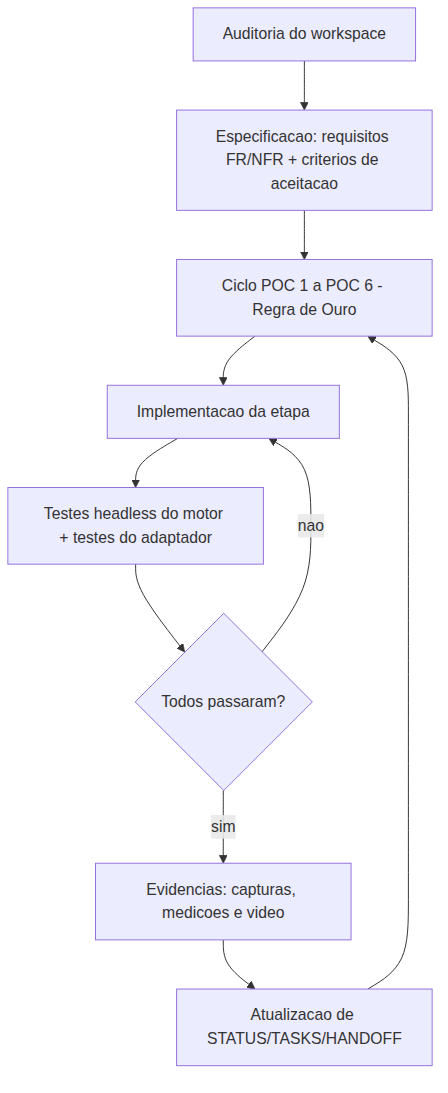
\includegraphics[width=0.85\textwidth]{05_processo.png}
\caption{Ciclo de desenvolvimento incremental adotado: especificação, implementação, verificação automatizada e registro de evidências.}
\label{fig:processo}
\end{figure}

O desenvolvimento foi assistido por agentes de inteligência artificial no
editor de código. Para que essa assistência permanecesse sob controle, os
documentos de especificação, regras e estado foram mantidos versionados e
foram tratados como a fonte de intenção: cada tarefa delegada a um agente
referenciava requisitos e critérios de aceitação explícitos. Um servidor MCP
\cite{mcp2026} expôs a cena do Blender à manipulação programática, o que
permitiu conduzir a modelagem 3D e a exportação também dentro do fluxo
assistido. A Figura~\ref{fig:arquitetura} (no
\autoref{cap:desenvolvimento}) mostra o resultado arquitetural desse processo.

\section{Ambiente de referência}
\label{sec:ambiente}

Todas as medições deste trabalho foram realizadas em uma única máquina de
referência, descrita na Tabela~\ref{tab:ambiente}. A escolha é deliberada:
o critério de projeto é a execução em computador pessoal sem GPU dedicada, e
por isso nenhuma medição utiliza hardware especializado.

% Tabela de ambiente de referência (usada no capítulo 4).
\begin{table}[htbp]
\centering
\caption{Ambiente de referência utilizado em todas as medições (verificado em 2026-09-10).}
\label{tab:ambiente}
\footnotesize
\begin{tabular}{@{}>{\raggedright\arraybackslash}p{4.4cm} >{\raggedright\arraybackslash}p{9.4cm}@{}}
\toprule
Item & Versão ou configuração \\
\midrule
Sistema operacional & Ubuntu 24.04.4 LTS (64 bits) \\
Processador & AMD Ryzen 7 5700U com Radeon Graphics \\
Memória principal & 30 GiB \\
GPU & GPU integrada AMD Radeon Graphics (sem GPU dedicada) \\
Motor de jogo & Godot 4.5 (\texttt{4.5.stable.official.876b29033}), renderizador \texttt{gl\_compatibility} \\
Modelagem 3D & Blender 5.2.1 LTS \\
Linguagem do adaptador & Python 3.12.3 \\
Bibliotecas do adaptador & FastAPI 0.141.1; Uvicorn 0.52.4; Pydantic 2.13.5; requests 2.34.2 \\
Inferência local & Ollama; modelo-alvo \texttt{llama3.2:3b} (não instalado no ambiente); validação realizada com \texttt{llama3.1:8b} \\
Formato de assets & glTF 2.0 binário (GLB) \\
Resolução de execução & 1280$\times$720 com sincronismo vertical (vsync) \\
\bottomrule
\end{tabular}
\par\vspace{2pt}{\footnotesize Fonte: elaborado pelo autor (2026); valores obtidos por comando na máquina de referência.}
\end{table}


O projeto mantém um passo de importação de recursos (modelos GLB e áudio)
executado por linha de comando, necessário na primeira execução de cada
cópia do repositório; a suíte de testes e as capturas também são executadas
por linha de comando, sem interface gráfica (quando aplicável) nem
intervenção manual. A descrição do repositório, dos comandos e da organização
dos diretórios está no \autoref{ap:repositorio}.

\section{Instrumentos e métricas}
\label{sec:instrumentos}

A Tabela de instrumentos resume as métricas coletadas, o instrumento
correspondente e a forma de coleta. Todas as métricas são produzidas por
execução real do sistema na máquina de referência; nenhuma é estimada.

\begin{quadro}[htbp]
\centering
\caption{Instrumentos de avaliação e métricas coletadas.}
\label{quad:instrumentos}
\footnotesize
\begin{tabular}{@{}>{\raggedright\arraybackslash}p{3.6cm} >{\raggedright\arraybackslash}p{4.2cm} >{\raggedright\arraybackslash}p{5.4cm}@{}}
\toprule
Métrica & Instrumento & Forma de coleta \\
\midrule
Verificações funcionais por etapa & Cenas de teste \emph{headless} do motor (uma por POC) & Execução de \texttt{tests/run\_all.sh}; contagem de verificações aprovadas impressa por cena \\
Testes de contrato da IA & Suíte do adaptador em Python & Execução por linha de comando contra o serviço local \\
Desempenho gráfico & Motor em execução com janela & Leitura de quadros por segundo do próprio motor, com sincronismo vertical, em 1280$\times$720 \\
Latência da conversa & Cronometragem de três execuções independentes & Chamada direta ao adaptador (partida fria), terminal no jogo e cliente em teste ao vivo; valores obtidos do relatório de execução e da captura de evidência \\
Complexidade do asset 3D & Inspeção programática do arquivo GLB & Contagem de nós, materiais e malhas de colisão por script \\
Evidências visuais & Arnês de captura do projeto & Execução com variáveis de ambiente que posicionam o jogador, opcionalmente concluem a missão e salvam imagens em 1280$\times$720 \\
\bottomrule
\end{tabular}
\par\vspace{2pt}{\footnotesize Fonte: elaborado pelo autor (2026).}
\end{quadro}

\section{Critérios de aceitação e rastreabilidade}
\label{sec:criterios}

Cada requisito funcional possui um critério de aceitação no formato
DADO\slash QUANDO\slash ENTÃO, escrito antes da implementação. A
Tabela~\ref{tab:aceitacao_resumo} (no \autoref{cap:resultados}) resume o
status de cada critério; o Quadro~\ref{quad:ca_exemplos} apresenta dois
exemplos representativos, um de cada subsistema crítico. A lista completa dos
requisitos e critérios está no \autoref{ap:requisitos}.

\begin{quadro}[htbp]
\centering
\caption{Exemplos de critérios de aceitação usados como contrato de implementação.}
\label{quad:ca_exemplos}
\footnotesize
\begin{tabular}{@{}>{\raggedright\arraybackslash}p{1.4cm} >{\raggedright\arraybackslash}p{11.6cm}@{}}
\toprule
ID & Critério (resumo) \\
\midrule
CA-009 & DADO que o serviço de IA está indisponível ou lento, QUANDO o jogador envia uma mensagem, ENTÃO o jogo exibe uma resposta de \emph{fallback} dentro do limite de tempo, sem travar. \\
CA-010 & DADO uma resposta do modelo, QUANDO a intenção não pertence ao conjunto permitido, ENTÃO ela é convertida para \texttt{NONE} e a resposta textual permanece válida. \\
\bottomrule
\end{tabular}
\par\vspace{2pt}{\footnotesize Fonte: elaborado pelo autor (2026), a partir da especificação do projeto.}
\end{quadro}

A rastreabilidade é mantida em duas matrizes. A primeira associa cada
objetivo específico desta monografia aos métodos e evidências correspondentes;
a segunda associa requisito, critério de aceitação, teste e evidência. Ambas
estão consolidadas no arquivo de rastreabilidade do projeto
(MONOGRAFIA\_RASTREABILIDADE.md) e resumidas no
\autoref{cap:resultados}.

\section{Procedimentos experimentais}
\label{sec:procedimentos}

Os procedimentos seguiram uma ordem fixa, executada ao final do
desenvolvimento e repetida a cada alteração relevante:

\begin{enumerate}
  \item \textbf{Verificação funcional:} execução completa da suíte
  \emph{headless} (etapas \poc{1} a \poc{6}) e da suíte do adaptador de IA,
  registrando o número de verificações e falhas de cada cena;
  \item \textbf{Verificação de integração ao vivo:} execução do jogo com o
  adaptador e o modelo local ativos, enviando uma pergunta real pelo terminal
  da IA e registrando a resposta e a latência;
  \item \textbf{Medição de latência:} três contextos independentes --- chamada
  direta ao adaptador em partida fria, mensagem pelo terminal com o jogo em
  execução e teste ao vivo do cliente ---, todos com o mesmo modelo local;
  \item \textbf{Medição de desempenho:} execução da cena completa em
  1280$\times$720 com sincronismo vertical, lendo os quadros por segundo
  reportados pelo motor;
  \item \textbf{Evidências visuais:} geração de capturas em poses
  pré-determinadas, incluindo o estado inicial, o estado após a missão
  concluída e o terminal da IA com a resposta do modelo;
  \item \textbf{Inspeção do artefato 3D:} medição programática do GLB
  exportado (nós, materiais, colisões e tamanho em disco).
\end{enumerate}

Os itens que exigem presença física ou julgamento humano --- operação de
mouse com captura de cursor, calibração do adaptador de joystick em hardware
real e o percurso completo do início ao fim por uma pessoa --- estão
declarados como pendentes de validação manual e não foram contabilizados como
concluídos.

\section{Ameaças à validade do método}
\label{sec:ameacas_metodo}

Quatro ameaças devem ser consideradas na leitura dos resultados. A primeira é
de \textbf{generalização}: trata-se de um estudo de caso único, com um
artefato construído por um único autor; os resultados não se generalizam
automaticamente para outros jogos, outros modelos de linguagem ou outras
máquinas. A segunda é de \textbf{medição}: as latências foram coletadas em
três execuções por contexto, sem repetição estatística; são indicativas, não
experimentais. A terceira é de \textbf{autoria}: o mesmo autor especificou,
implementou e avaliou o artefato, o que aumenta o risco de viés de confirmação;
a mitigação adotada é externa ao autor --- critérios escritos antes da
implementação, testes automatizados executáveis por terceiros e artefatos
públicos. A quarta é de \textbf{ambiente}: os resultados de desempenho valem
para a máquina de referência; o capítulo de discussão registra duas
particularidades de ambiente que afetaram a experiência de uso e que outros
projetos podem encontrar (confinamento de pacote do motor e estado de áudio
por aplicativo).

\section{Planejado versus executado}
\label{sec:planejado_executado}

O trabalho distingue explicitamente o que foi planejado do que foi executado.
O Quadro~\ref{quad:planejado} apresenta a distinção por componente; a coluna
de status registra o que permanece aberto, sem conversão de intenção em
resultado.

\begin{quadro}[htbp]
\centering
\caption{Planejado versus executado, por componente do projeto.}
\label{quad:planejado}
\footnotesize
\begin{tabular}{@{}>{\raggedright\arraybackslash}p{4.0cm} >{\raggedright\arraybackslash}p{4.6cm} >{\raggedright\arraybackslash}p{4.2cm}@{}}
\toprule
Componente & Planejado & Executado e status \\
\midrule
Jogo (etapas \poc{1}--\poc{6}) & Seis provas de conceito demonstráveis & Executado; suíte automatizada verde \\
IA local & Conversa com modelo local e \emph{fallback} & Executado com \texttt{llama3.1:8b}; modelo-alvo \texttt{llama3.2:3b} não instalado (aberto) \\
Desempenho & Executar sem GPU dedicada & Executado a 60 FPS (vsync) na máquina de referência \\
Medições de latência & Três contextos independentes & Executado (uma execução por contexto) \\
Evidências visuais & Capturas em poses controladas e vídeo & Executado (capturas e vídeo de 68 s) \\
Validação de hardware & Operar com joystick físico e mouse & Pendente (validação manual) \\
Percurso humano (CA-013) & Jogo completo por uma pessoa & Pendente (validação manual) \\
Empacotamento (FR-033) & Executável independente & Bloqueado por ausência de modelos de exportação no ambiente \\
Estudo com usuários & Fora do escopo declarado & Não realizado (trabalho futuro) \\
\bottomrule
\end{tabular}
\par\vspace{2pt}{\footnotesize Fonte: elaborado pelo autor (2026).}
\end{quadro}

\section{Considerações do capítulo}
\label{sec:consideracoes_metodos}

O método combina elementos de engenharia de software --- especificação,
rastreabilidade, testes automatizados --- com os procedimentos de medição
descritos nesta seção. É esse conjunto que sustenta a afirmação, repetida ao
longo do trabalho, de que cada número apresentado possui origem verificável:
ele foi produzido por um comando, por uma execução ou por uma medição, e não
por estimativa.

\chapter{Desenvolvimento}
\label{cap:desenvolvimento}

Este capítulo descreve como o Laboratório 404 foi construído: a arquitetura
geral, a especificação que organizou o trabalho e o desenvolvimento de cada
prova de conceito, com as decisões de engenharia relevantes e os defeitos
encontrados e corrigidos. O capítulo segue a ordem cronológica do projeto,
que é também a ordem de dependência entre os subsistemas.

\section{Visão geral da arquitetura}
\label{sec:arquitetura}

O sistema é composto por quatro blocos: o \textbf{jogo} (motor Godot, com
\emph{gameplay}, física, interface, áudio e persistência); os \textbf{assets
3D} (modelados no Blender e exportados em GLB); o \textbf{adaptador de IA}
(serviço local em Python que valida e media a conversa); e a \textbf{IA}
propriamente dita (modelo de linguagem executado localmente pelo Ollama). A
Figura~\ref{fig:arquitetura} apresenta o conjunto.

\begin{figure}[htbp]
\centering
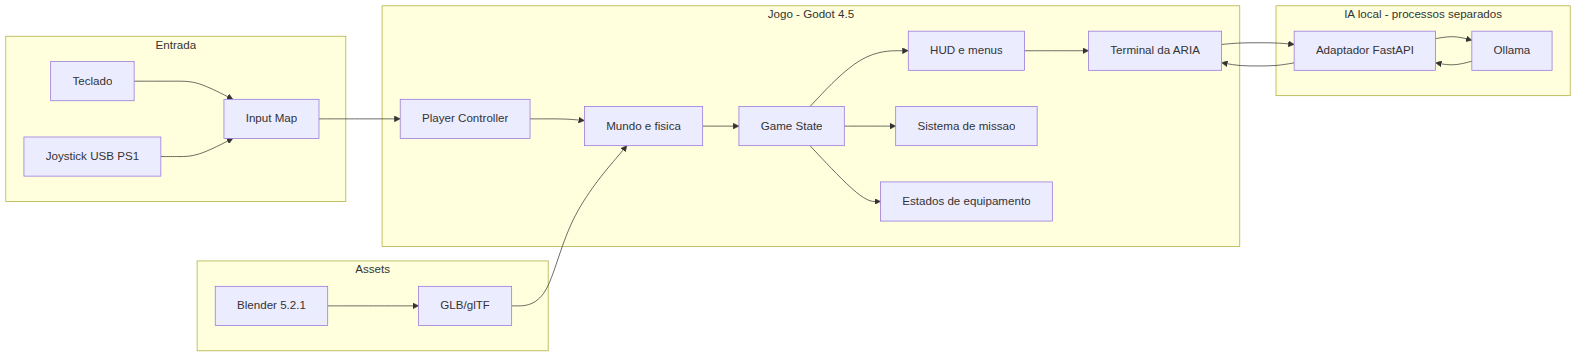
\includegraphics[width=0.95\textwidth]{01_arquitetura.png}
\caption{Arquitetura do Laboratório 404: o jogo consome assets do Blender e ações de entrada; a IA vive em processos separados, atrás de um adaptador que valida entrada e saída.}
\label{fig:arquitetura}
\end{figure}

Duas decisões estruturais merecem destaque. A primeira é manter a IA
\emph{fora} do processo do jogo: se o adaptador ou o modelo falham, o jogo
continua jogável e responde com textos de \emph{fallback}. A segunda é tratar
o adaptador como fronteira de segurança: é nele que a entrada é validada, que
o contexto do jogo é injetado no \emph{prompt} e que a saída do modelo é
reduzida a texto e a uma intenção pertencente a um conjunto finito.

\section{Especificação e organização incremental}
\label{sec:especificacao}

Antes da implementação, o projeto foi especificado com requisitos funcionais
(FR) e não funcionais (NFR), critérios de aceitação no formato
DADO/QUANDO/ENTÃO e uma matriz de rastreabilidade que associa cada requisito
ao teste correspondente. Os requisitos foram agrupados por prova de conceito,
e cada grupo tinha um critério de avanço explícito: a etapa só era considerada
concluída com a suíte verde e as evidências registradas. O
\autoref{ap:requisitos} reproduz a especificação consolidada; o
\autoref{ap:testes} detalha a suíte.

\section{\poc{1} --- Fundação jogável}
\label{sec:poc1}

O primeiro incremento estabeleceu o esqueleto do jogo: um jogador que se
movimenta, uma câmera, um HUD mínimo, menu de pausa e --- decisão que se
provou estruturante --- um mapa de entrada inteiramente baseado em ações
semânticas.

\subsection{Entrada semântica e diagnóstico de controles}

O jogo consome ações nomeadas (por exemplo, \texttt{move\_forward},
\texttt{look\_right}, \texttt{interact}, \texttt{pause}) e nunca índices
numéricos de botão ou eixo. A razão é prática: adaptadores USB convertem
controles de maneiras distintas, e um índice fixo deixa de funcionar quando o
adaptador muda. Com ações semânticas, o mapeamento físico fica isolado na
configuração do motor. O Quadro~\ref{quad:input} ilustra o padrão usado em
todo o \emph{gameplay}.

\begin{quadro}[htbp]
\centering
\caption{Padrão de leitura de entrada usado no gameplay (GDScript).}
\label{quad:input}
\begin{verbatim}
var direcao := Input.get_vector(
    "move_left", "move_right",
    "move_forward", "move_backward")
# NUNCA usar indices crus, como Input.is_joy_button_pressed(0, 1)
\end{verbatim}
\par\vspace{2pt}{\footnotesize Fonte: elaborado pelo autor (2026), a partir do código do projeto.}
\end{quadro}

Para calibrar adaptadores desconhecidos, o projeto inclui uma tela de
diagnóstico de entrada que lista os dispositivos conectados, os eixos e os
botões em tempo real, com zona morta configurável (padrão de 0,15) e
tratamento de conexão e desconexão a quente (\emph{hotplug}) sem interromper a
execução. Essa tela é a única parte do projeto autorizada a ler índices
numéricos; o \emph{gameplay}, jamais.

\subsection{Jogador, câmera, HUD e pausa}

O jogador é um corpo com física que respeita gravidade e colisão. A câmera é
controlada por mouse e, quando o adaptador expõe os eixos do analógico
direito, por este. O HUD exibe o objetivo corrente e o convite de interação
contextual; o menu de pausa (\texttt{Esc}/\emph{Start}) dá acesso ao
diagnóstico de entrada, ao salvamento e à saída. Essas funcionalidades
correspondem aos requisitos FR-002 a FR-006 e foram verificadas
automaticamente (critérios CA-001 a CA-005), com duas ressalvas manuais: o
uso do mouse com captura de cursor e a operação física do joystick.

\section{\poc{2} --- Laboratório funcional}
\label{sec:poc2}

O segundo incremento transformou o esqueleto em um laboratório: uma sala
modelada no Blender, interação por proximidade, inventário, missão e estados
de equipamento.

\subsection{Pipeline de assets: do Blender ao jogo}
\label{sec:pipeline_assets}

Os assets 3D seguem convenções fixas que tornaram a integração previsível:
1 unidade do Blender equivale a 1 metro; as transformações são aplicadas antes
da exportação; os objetos são nomeados por função (Quadro~\ref{quad:prefixos});
e a colisão é embutida no próprio asset por meio do sufixo \texttt{-col} ---
o importador do motor converte essas malhas em corpos estáticos, mantendo a
malha visível original apenas para renderização.

\begin{quadro}[htbp]
\centering
\caption{Prefixos de nomenclatura adotados na modelagem.}
\label{quad:prefixos}
\footnotesize
\begin{tabular}{@{}>{\raggedright\arraybackslash}p{2.0cm} >{\raggedright\arraybackslash}p{11.0cm}@{}}
\toprule
Prefixo & Uso \\
\midrule
\texttt{ENV\_} & arquitetura (paredes, piso, teto, estruturas) \\
\texttt{PROP\_} & equipamento ou objeto cenográfico \\
\texttt{INT\_} & objeto interativo \\
\texttt{COL\_} & colisor auxiliar \\
\texttt{FX\_} & efeito visual \\
\texttt{NPC\_} & personagem \\
\texttt{DEC\_} & decoração \\
\bottomrule
\end{tabular}
\par\vspace{2pt}{\footnotesize Fonte: elaborado pelo autor (2026), a partir das convenções do projeto.}
\end{quadro}

A exportação é feita por script, com parâmetros fixos: formato binário GLB,
transformações aplicadas, eixo vertical convertido, e \emph{exclusão} de
câmeras e luzes do arquivo (a iluminação é reconstruída no motor, o que
permite ajustá-la sem reexportar). O Quadro~\ref{quad:export} reproduz a
chamada de exportação de referência. Depois de cada exportação, o projeto
executa a importação de recursos por linha de comando e a suíte de testes,
garantindo que o asset novo não quebrou nenhuma verificação.

\begin{quadro}[htbp]
\centering
\caption{Exportação de referência do asset 3D (script do Blender).}
\label{quad:export}
\begin{verbatim}
bpy.ops.export_scene.gltf(
    filepath="assets/lab404/lab_sala_poc2.glb",
    export_format='GLB', export_apply=True, export_yup=True,
    export_cameras=False, export_lights=False)
\end{verbatim}
\par\vspace{2pt}{\footnotesize Fonte: elaborado pelo autor (2026), a partir do pipeline do projeto.}
\end{quadro}

O asset final da sala contém 342 nós, 37 materiais e 35 nós de colisão,
totalizando 1.018,7~KB --- números obtidos por inspeção programática do
arquivo, não por estimativa. O emissivo dos materiais usa a extensão
\texttt{KHR\_materials\_emissive\_strength} do glTF, o que permitiu acender
telas e sinalizações com intensidade controlada, sem estourar para branco no
renderizador compatível.

\subsection{A sala e o detalhamento visual}
\label{sec:sala}

A sala do laboratório foi modelada a partir de uma referência visual de
ambiente industrial e refinada iterativamente. A
Figura~\ref{fig:referencia} mostra a referência de arte usada e a
Figura~\ref{fig:sala_geral} mostra o resultado em jogo, no estado inicial ---
energia isolada, iluminação de emergência e a missão pendente no HUD.

\begin{figure}[htbp]
\centering
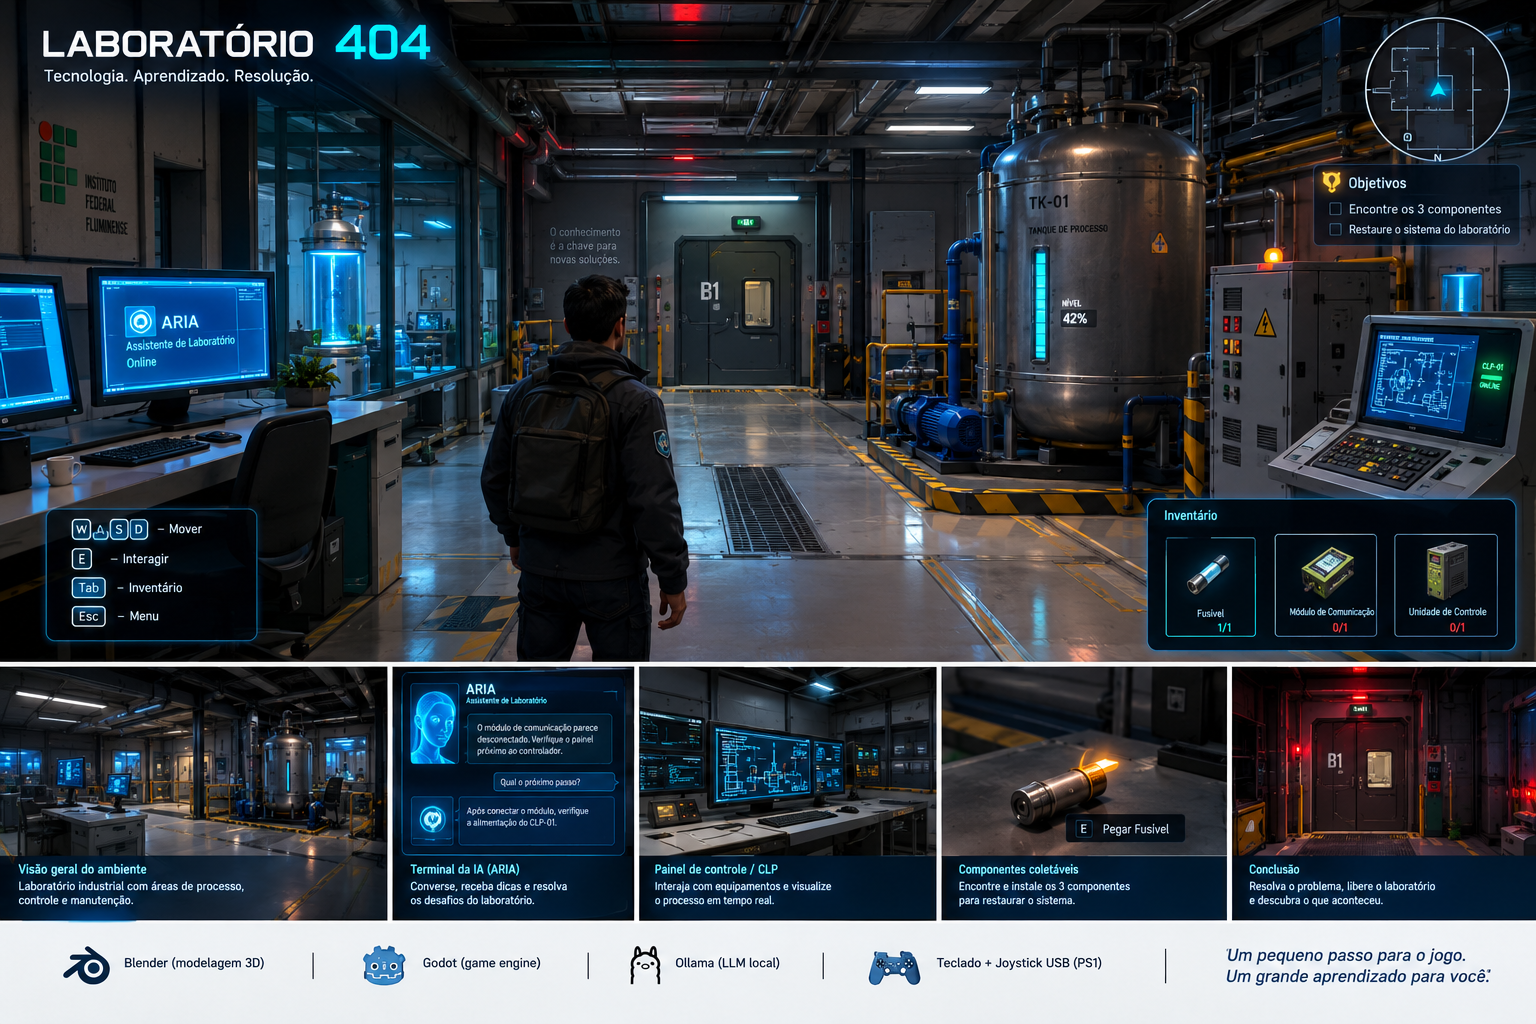
\includegraphics[width=0.8\textwidth]{referencia_arte.png}
\caption{Referência visual utilizada para a reconstrução da sala (imagem de referência adotada no projeto).}
\label{fig:referencia}
\end{figure}

\begin{figure}[htbp]
\centering
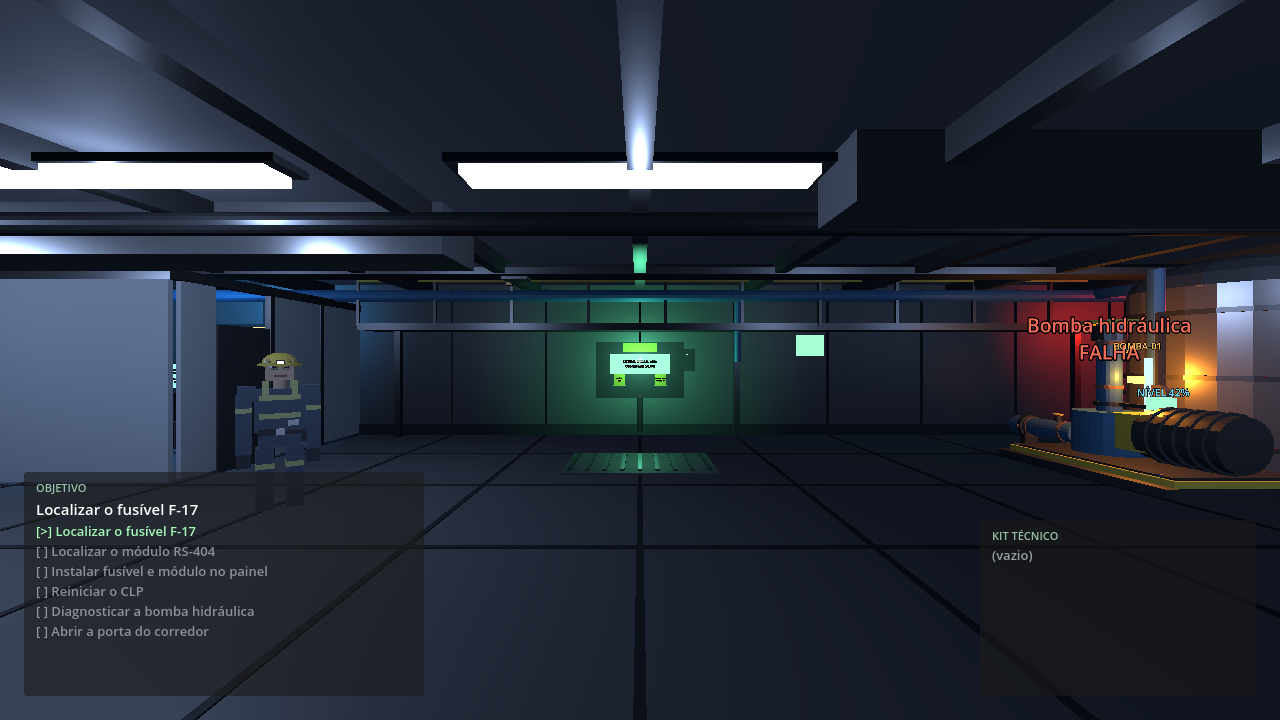
\includegraphics[width=0.8\textwidth]{sala_geral.png}
\caption{Sala do Laboratório 404 no estado inicial: energia isolada, iluminação de emergência, técnico (NPC) à esquerda e bomba em falha. Captura do jogo em 1280$\times$720.}
\label{fig:sala_geral}
\end{figure}

O detalhamento seguiu um princípio econômico: cada elemento adicional precisava
ter função visual ou narrativa. O CLP ganhou ranhuras de ventilação e quatro
LEDs de status que piscam em períodos distintos; o painel de encaixe recebeu
faixas zebradas de perigo, triângulo de alerta elétrico, esquema de fiação e
molduras dos slots; a bomba recebeu braçadeiras, apoios ancorados ao piso,
longarinas com parafusos sextavados, manômetro analógico com ponteiro e
válvulas de alívio; e a bancada de trabalho recebeu luminária própria. As
Figuras~\ref{fig:clp} a \ref{fig:bancada} ilustram esse conjunto.

\begin{figure}[htbp]
\centering

\includegraphics[width=0.72\textwidth]{clp.png}
\caption{Estação do CLP, com ranhuras de ventilação, LEDs de status e diagrama \emph{ladder} na tela.}
\label{fig:clp}
\end{figure}

\begin{figure}[htbp]
\centering
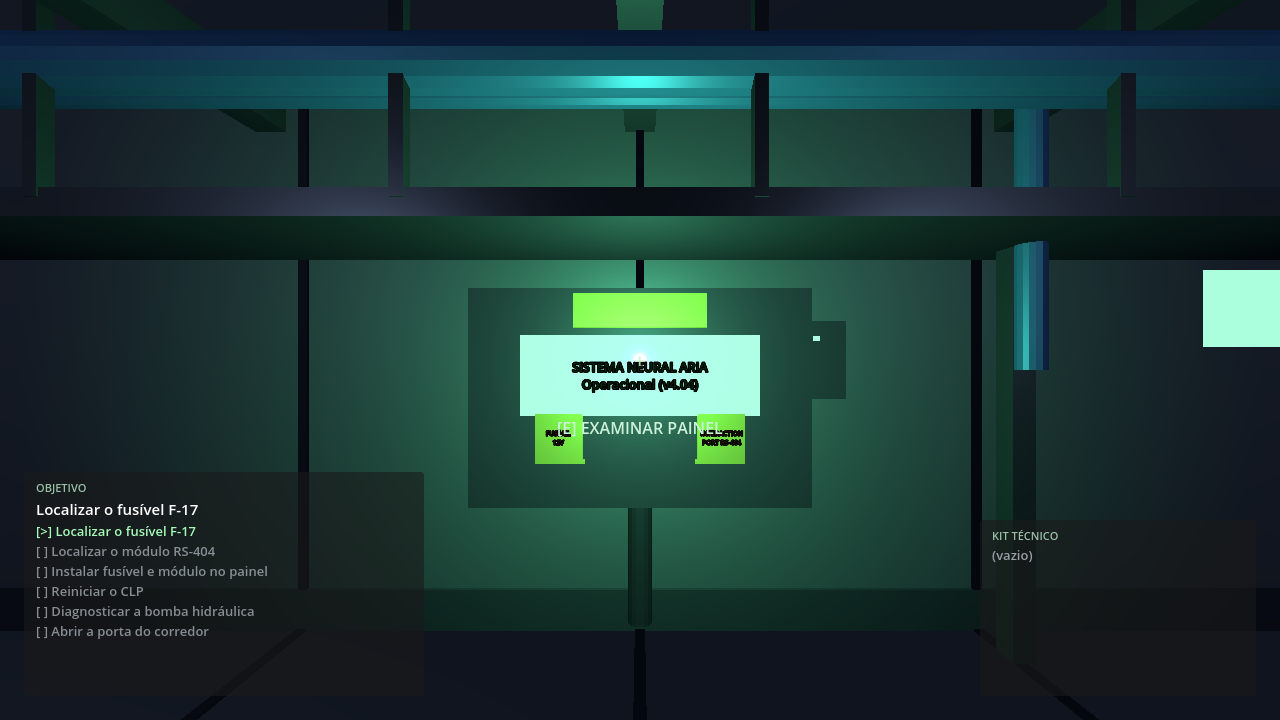
\includegraphics[width=0.72\textwidth]{painel.png}
\caption{Painel de encaixe, com sinalização de perigo, esquema de fiação e slots para o fusível e o módulo.}
\label{fig:painel}
\end{figure}

\begin{figure}[htbp]
\centering

\includegraphics[width=0.72\textwidth]{bomba.png}
\caption{Conjunto da bomba hidráulica, com manômetro, tubulações e ancoragens mecânicas, em estado de falha.}
\label{fig:bomba}
\end{figure}

\begin{figure}[htbp]
\centering
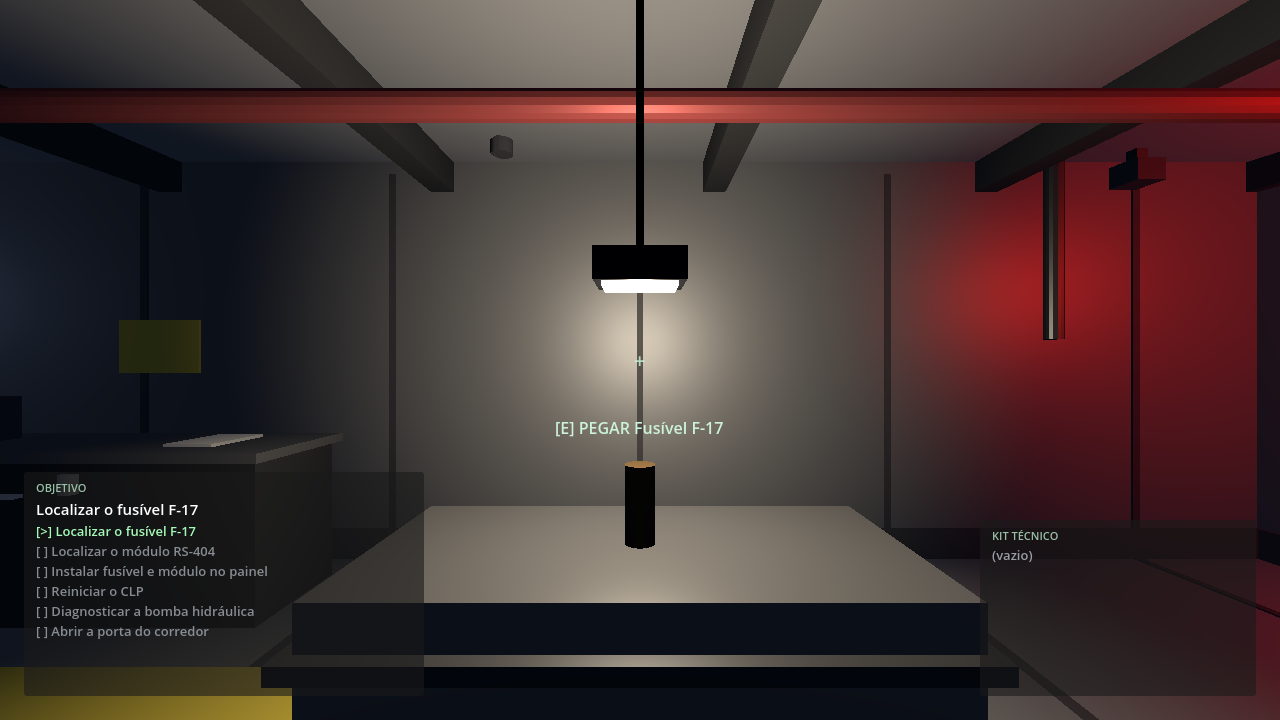
\includegraphics[width=0.72\textwidth]{bancada.png}
\caption{Bancada de trabalho com luminária dedicada, onde está o item coletável inicial.}
\label{fig:bancada}
\end{figure}

Duas decisões técnicas do detalhamento merecem registro porque contrariam
expectativas comuns de quem vem da modelagem tradicional: LEDs que piscam
\emph{não} podem ser animados no glTF (o formato anima apenas translação,
rotação e escala, não emissão de material --- de modo que o piscar é feito por
script no motor, alternando a visibilidade dos nós dos LEDs); e textos de
tela são implementados como nós de texto do próprio motor, sobre a tela
emissiva do modelo, evitando dependência de fontes dentro do GLB e
permitindo ajustes de idioma sem reexportar o asset.

\subsection{Interação, inventário e missão}
\label{sec:interacao}

A interação é um sistema desacoplado: um raio de proximidade detecta objetos
interativos, exibe o convite contextual no HUD e, quando a ação de interagir é
acionada, emite um sinal que o objeto trata. O inventário é diegético (um kit
técnico), em vez de uma grade abstrata: o jogador coleta o fusível F-17, o
módulo RS-404 e uma chave de manutenção, e os instala nos pontos
correspondentes da sala.

A missão principal, \texttt{RESTAURAR\_COMUNICACAO}, encadeia seis passos
dependentes (Figura~\ref{fig:missao}): localizar o fusível, localizar o
módulo, instalar ambos no painel, reiniciar o CLP, diagnosticar a bomba e
abrir a porta do corredor. Cada passo só é aceito quando o anterior está
concluído, e o HUD reflete o avanço. O encadeamento é o que dá ao jogo sua
estrutura didática: o jogador percorre uma sequência de diagnóstico
semelhante à de um atendimento real.

\begin{figure}[htbp]
\centering
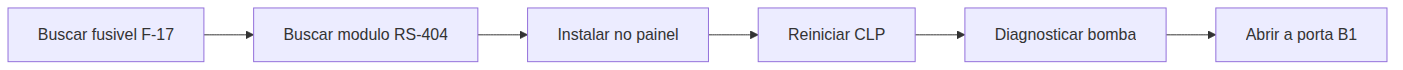
\includegraphics[width=0.95\textwidth]{04_missao.png}
\caption{Missão principal em seis passos dependentes e ordenados.}
\label{fig:missao}
\end{figure}

\subsection{Estados de equipamento}
\label{sec:estados}

Os equipamentos possuem uma máquina de estados explícita --- desligado,
falha, pronto e em operação --- serializável e independente da interface
(Figura~\ref{fig:estados}). A escolha por um estado explícito, em vez de
sinalizações dispersas, permitiu dois efeitos diretos: o mundo (luzes, NPC,
tom da IA) reage ao estado sem conhecer detalhes de implementação, e o
progresso do jogador pode ser salvo e restaurado com fidelidade.

\begin{figure}[htbp]
\centering
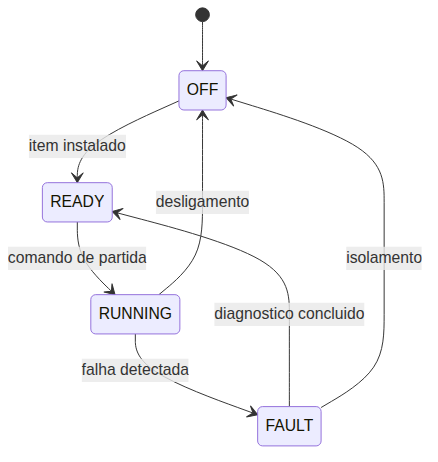
\includegraphics[width=0.72\textwidth]{03_estados_equipamento.png}
\caption{Máquina de estados dos equipamentos, serializável e independente da interface.}
\label{fig:estados}
\end{figure}

\subsection{Porta B1: um defeito visual e sua correção}
\label{sec:porta}

A porta do corredor --- obstáculo final da missão --- apresentou um defeito
instrutivo. No asset original, a folha da porta era composta por várias malhas
soltas; apenas a malha de colisão estava vinculada ao mecanismo de abertura.
O resultado visível era um paradoxo: a porta abria logicamente (o jogador
passava), mas o visual da folha permanecia fechado no vão. A correção foi
feita em duas frentes: no Blender, as malhas decorativas (reforço, visor e
placa) foram tornadas filhas do objeto da porta, e no jogo o mecanismo passou
a elevar a folha inteira em 2,15~m e a ocultá-la ao final do curso. As
Figuras~\ref{fig:porta_fechada} e \ref{fig:porta_aberta} mostram o antes e o
depois; os testes ganharam verificações específicas (a folha deve conter os
três detalhes como filhos e subir mais de 1,5~m).

\begin{figure}[htbp]
\centering
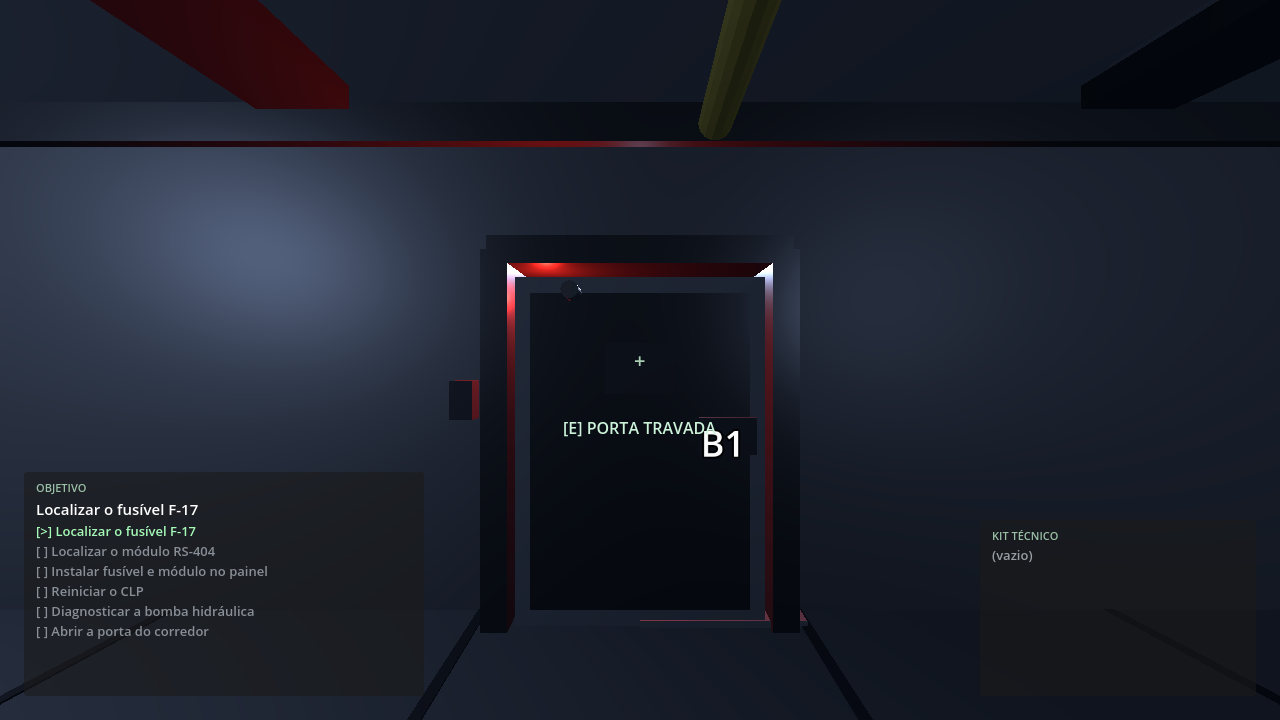
\includegraphics[width=0.72\textwidth]{porta_fechada.png}
\caption{Porta B1 fechada, antes de a missão ser concluída.}
\label{fig:porta_fechada}
\end{figure}

\begin{figure}[htbp]
\centering
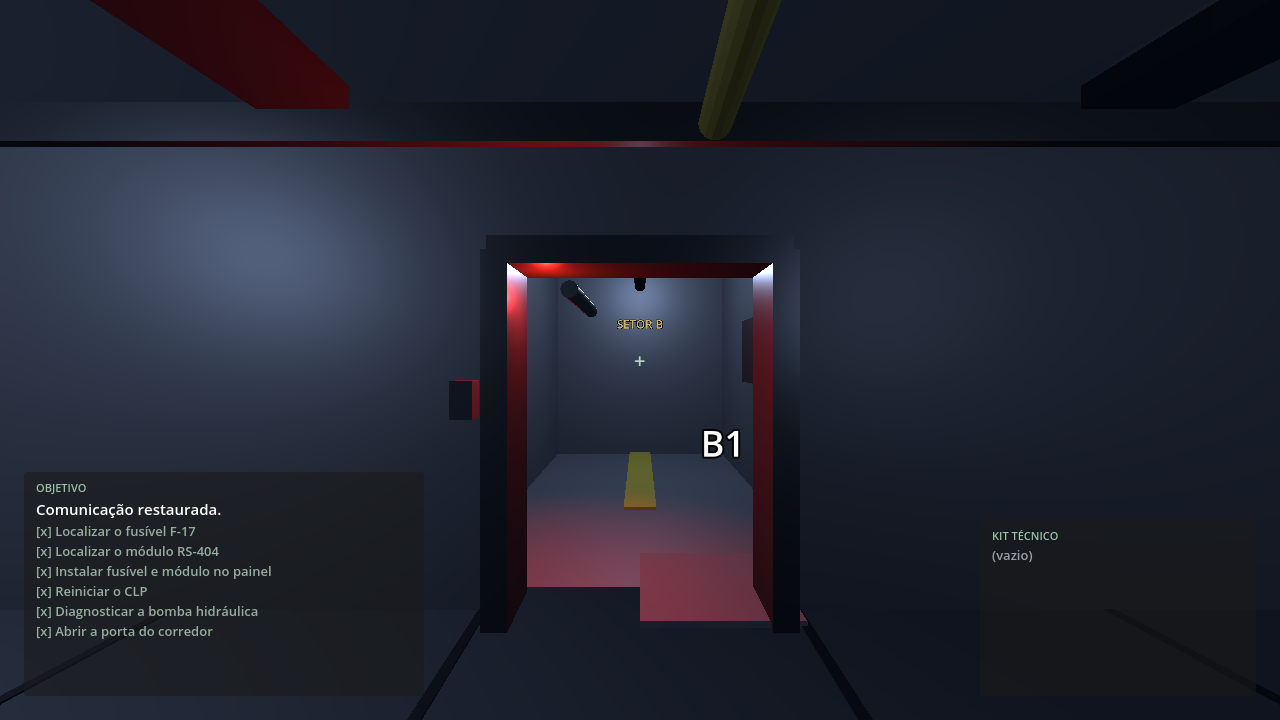
\includegraphics[width=0.72\textwidth]{porta_aberta.png}
\caption{Porta B1 aberta após a missão: a folha sobe e libera o vão do corredor.}
\label{fig:porta_aberta}
\end{figure}

Dois detalhes adicionais merecem registro no detalhamento dos equipamentos: o
esquema de fiação serigrafado do painel foi reposicionado na margem direita
(na posição original, ficava escondido atrás da tela) e o pato de borracha da
bancada --- um elemento decorativo --- precisou ser elevado acima da
superfície de colisão da bancada, que é mais alta que a superfície visível.
As Figuras~\ref{fig:det_painel} a \ref{fig:det_bomba} ilustram o nível de
detalhe alcançado.

\begin{figure}[htbp]
\centering
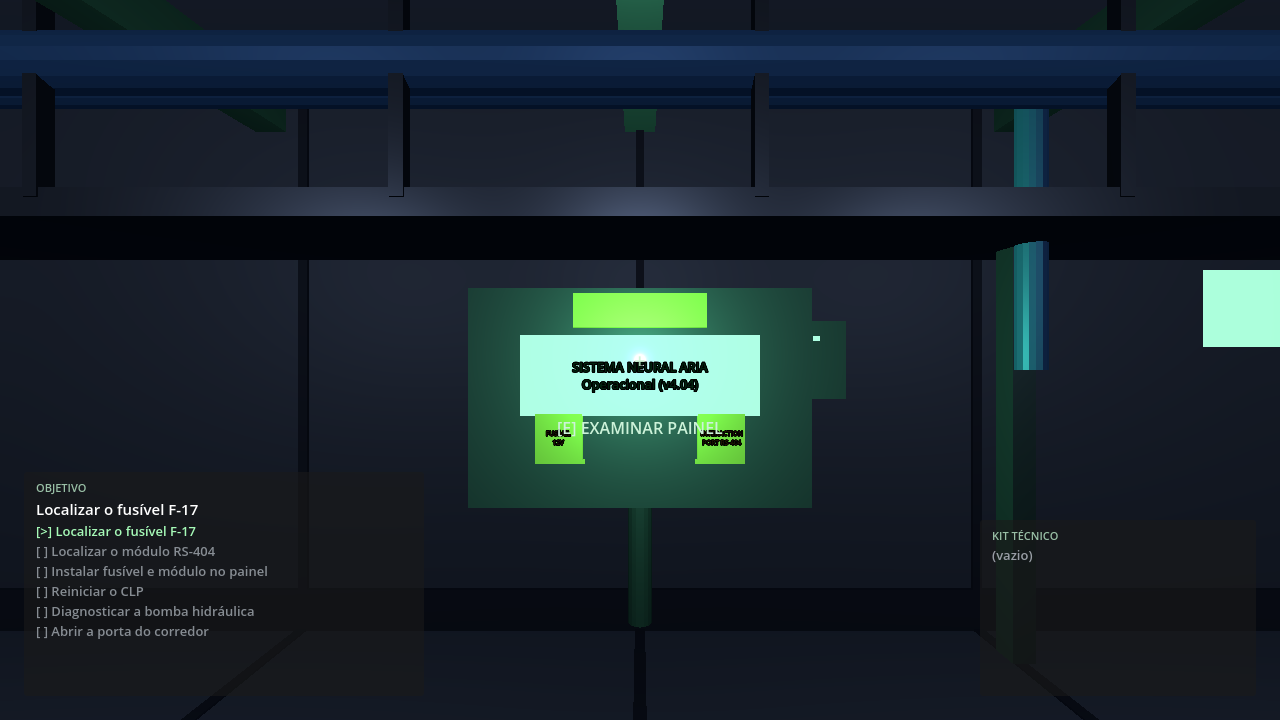
\includegraphics[width=0.72\textwidth]{detalhe_painel.png}
\caption{Detalhe do painel: faixas de perigo, triângulo de alerta, esquema de fiação e molduras dos slots.}
\label{fig:det_painel}
\end{figure}

\begin{figure}[htbp]
\centering
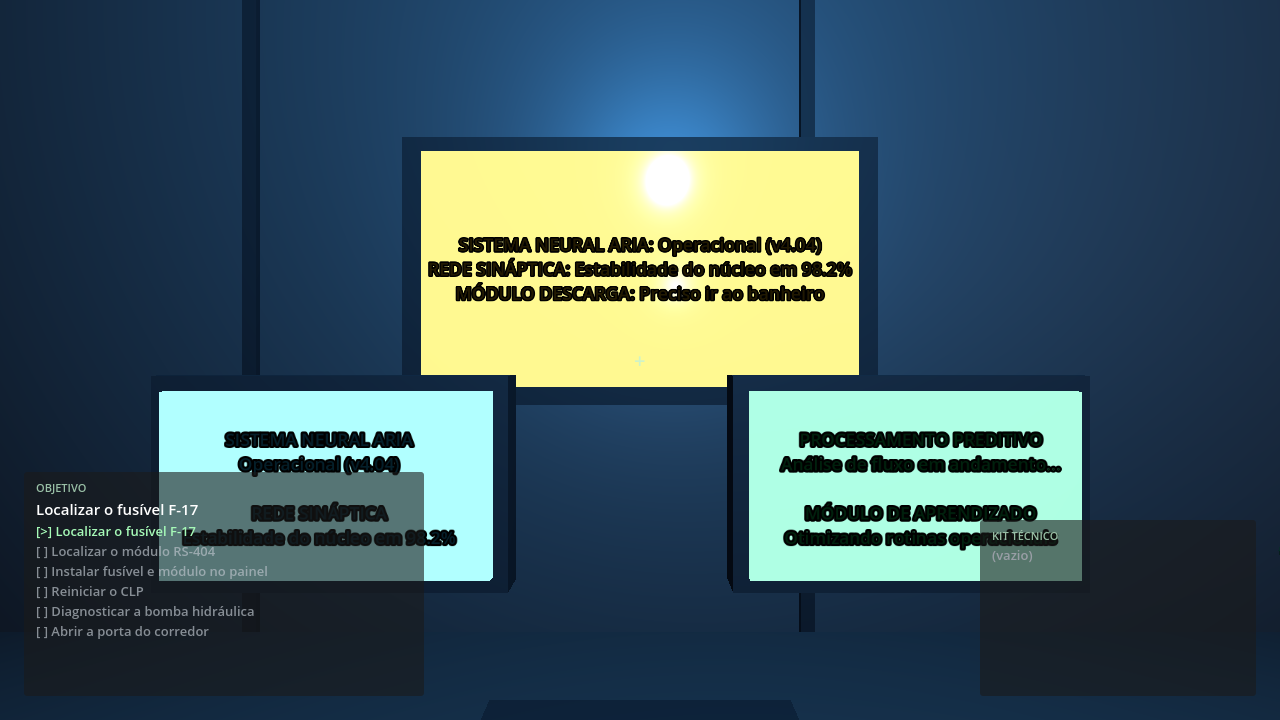
\includegraphics[width=0.72\textwidth]{detalhe_telas.png}
\caption{Detalhe das telas: conteúdos em português exibidos sobre as superfícies emissivas.}
\label{fig:det_telas}
\end{figure}

\begin{figure}[htbp]
\centering
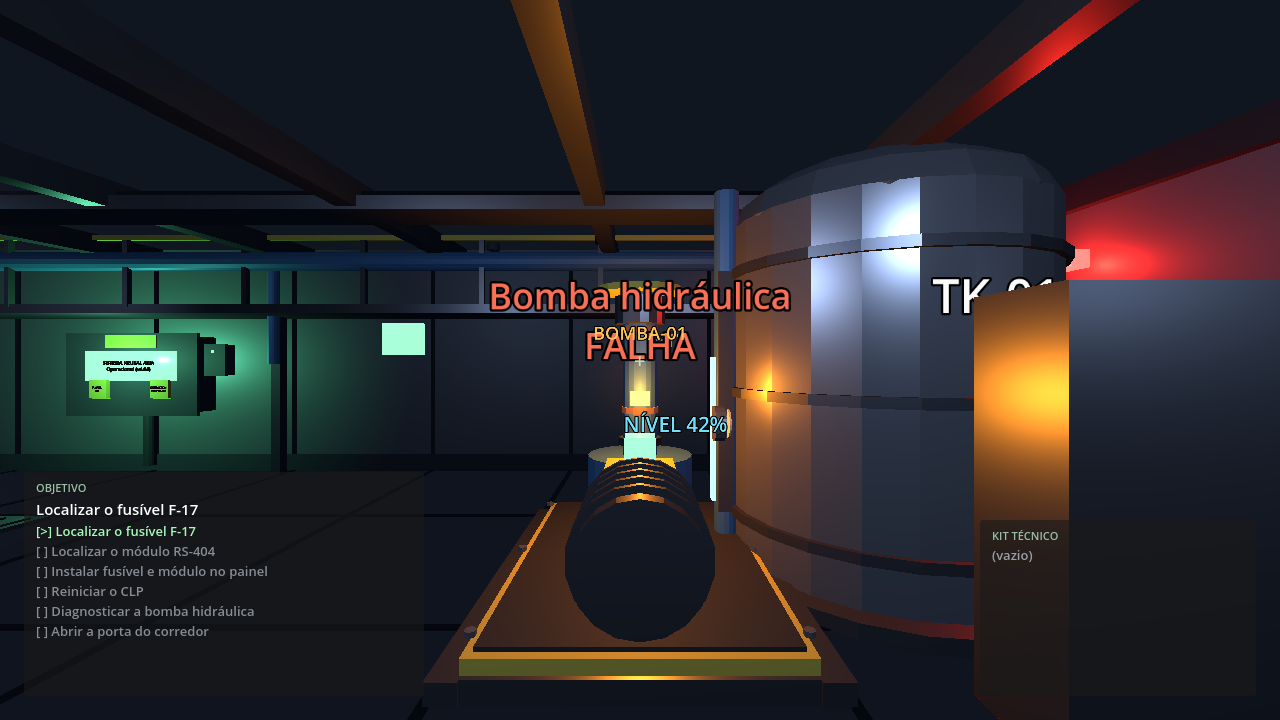
\includegraphics[width=0.72\textwidth]{detalhe_bomba.png}
\caption{Detalhe da bomba: braçadeiras, apoios, parafusos sextavados e manômetro.}
\label{fig:det_bomba}
\end{figure}

\section{\poc{3} --- \aria{}: IA local com intenções restritas}
\label{sec:poc3}

O terceiro incremento adicionou a personagem de IA. É o subsistema em que as
decisões de segurança mais importam, e por isso ele é descrito com detalhe.

\subsection{Fluxo de uma mensagem}
\label{sec:fluxo_mensagem}

A Figura~\ref{fig:fluxo} mostra o caminho de uma mensagem. O jogador digita
no terminal do jogo; o cliente (em GDScript) envia um JSON para o adaptador
local; o adaptador valida a entrada, monta o \emph{prompt} com a
personalidade versionada e o estado do jogo, chama o modelo e valida a
resposta antes de devolvê-la. Cada elo da cadeia pode falhar de forma segura:
o pior caso é um texto de \emph{fallback}, nunca um travamento ou uma ação não
prevista.

\begin{figure}[htbp]
\centering
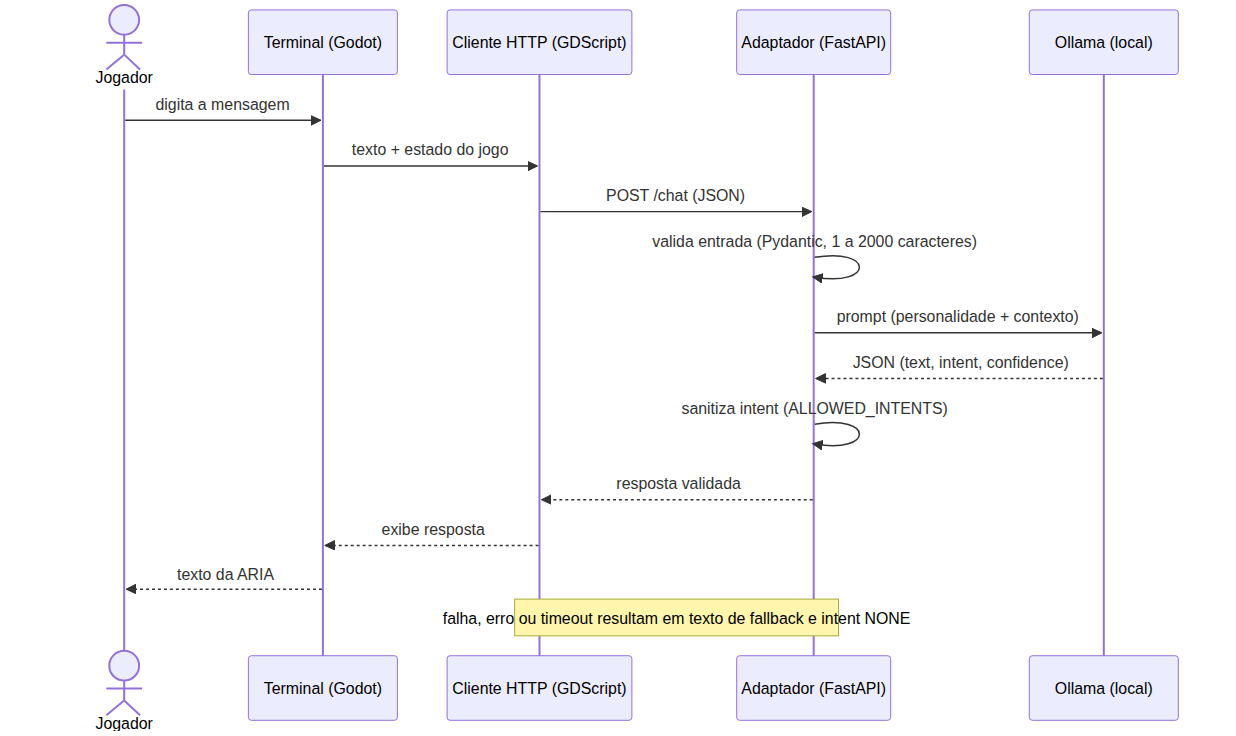
\includegraphics[width=0.95\textwidth]{02_fluxo_conversa.png}
\caption{Cadeia completa de uma mensagem até a resposta: validação em duas camadas e resposta de fallback em caso de falha.}
\label{fig:fluxo}
\end{figure}

\subsection{Contrato de dados}
\label{sec:contrato}

O adaptador expõe um único ponto de conversa e um ponto de verificação de
saúde. A entrada exige mensagem não vazia de até 2000 caracteres e um
dicionário opcional com o estado do jogo; a saída é sempre um objeto com
texto, intenção, alvo opcional, confiança e erro opcional. O
Quadro~\ref{quad:contrato} reproduz o contrato essencial.

\begin{quadro}[htbp]
\centering
\caption{Contrato de dados do adaptador de IA (resumo).}
\label{quad:contrato}
\begin{verbatim}
POST /chat
  request:  {"message": "A bomba nao liga.",
             "game_state": {"bomba": "FAULT", "energia": 62}}
  response: {"text": "...", "intent": "DIAGNOSE",
             "target": "PROP_Bomba", "confidence": 0.94}
validacao: 422 para entrada invalida;
           falha/timeout do modelo => texto de fallback, intent NONE
\end{verbatim}
\par\vspace{2pt}{\footnotesize Fonte: elaborado pelo autor (2026), a partir do adaptador do projeto.}
\end{quadro}

A validação de entrada usa modelos de dados declarativos (Pydantic), o que
garante que nenhuma mensagem fora dos limites chega ao modelo. A validação de
saída é a parte mais importante do desenho: o texto gerado é aceito, mas a
intenção só sobrevive se pertencer ao conjunto permitido --- caso contrário,
é convertida para \texttt{NONE}. A mesma sanitização é repetida no cliente do
jogo, de modo que as duas pontas precisam concordar. O
Quadro~\ref{quad:intents} reproduz o conjunto e a regra.

\begin{quadro}[htbp]
\centering
\caption{Conjunto de intenções permitidas e regra de sanitização (adaptador).}
\label{quad:intents}
\begin{verbatim}
ALLOWED_INTENTS = {"HINT", "DIAGNOSE", "LORE", "STATUS", "NONE"}

def sanitize_intent(valor):
    # remove ruido, normaliza e converte para maiusculas
    candidato = re.sub(r"[^A-Za-z]", "", str(valor or "")).upper()
    return candidato if candidato in ALLOWED_INTENTS else "NONE"
\end{verbatim}
\par\vspace{2pt}{\footnotesize Fonte: elaborado pelo autor (2026), a partir do código do adaptador.}
\end{quadro}

\subsection{Personalidade versionada}
\label{sec:personalidade}

A personalidade da IA não está espalhada pelo código: ela vive em um arquivo
de configuração versionado, com identidade, regras de conduta, tons de voz
(neutra, impaciente, preocupada), saudação e texto de \emph{fallback}. Duas
regras desse arquivo materializam o desenho de segurança adotado: a IA
\emph{não executa comandos, não controla portas, energia nem física}; e nunca
inventa componentes, códigos ou procedimentos inexistentes no laboratório.
O tom pode ser alterado pelo estado do jogo --- por exemplo, quando o jogador
ignora um alerta, a IA responde de forma mais curta e seca ---, o que dá
coerência afetiva à ficção sem ampliar seu poder de ação.

\subsection{Limites de tempo e resposta de segurança}
\label{sec:fallback}

O adaptador aguarda o modelo por até 30 segundos; o cliente no jogo espera um
pouco mais (35 segundos) para acomodar a variabilidade de um modelo local.
Esgotado o prazo --- ou ocorrendo qualquer erro de rede, de validação ou de
modelo ---, a resposta devolvida é o texto de \emph{fallback} com intenção
\texttt{NONE}. Essa é a garantia que sustenta o requisito CA-009: o jogo
nunca trava por causa da IA.

\subsection{No jogo: terminal e estação}
\label{sec:terminal}

No jogo, a conversa acontece em um terminal com histórico de mensagens e
entrada de texto, acessível ao interagir com a estação da IA
(Figura~\ref{fig:aria_estacao}). A estação também exibe uma leitura de status
própria, com identificação da versão do núcleo e do canal de comunicação.

\begin{figure}[htbp]
\centering
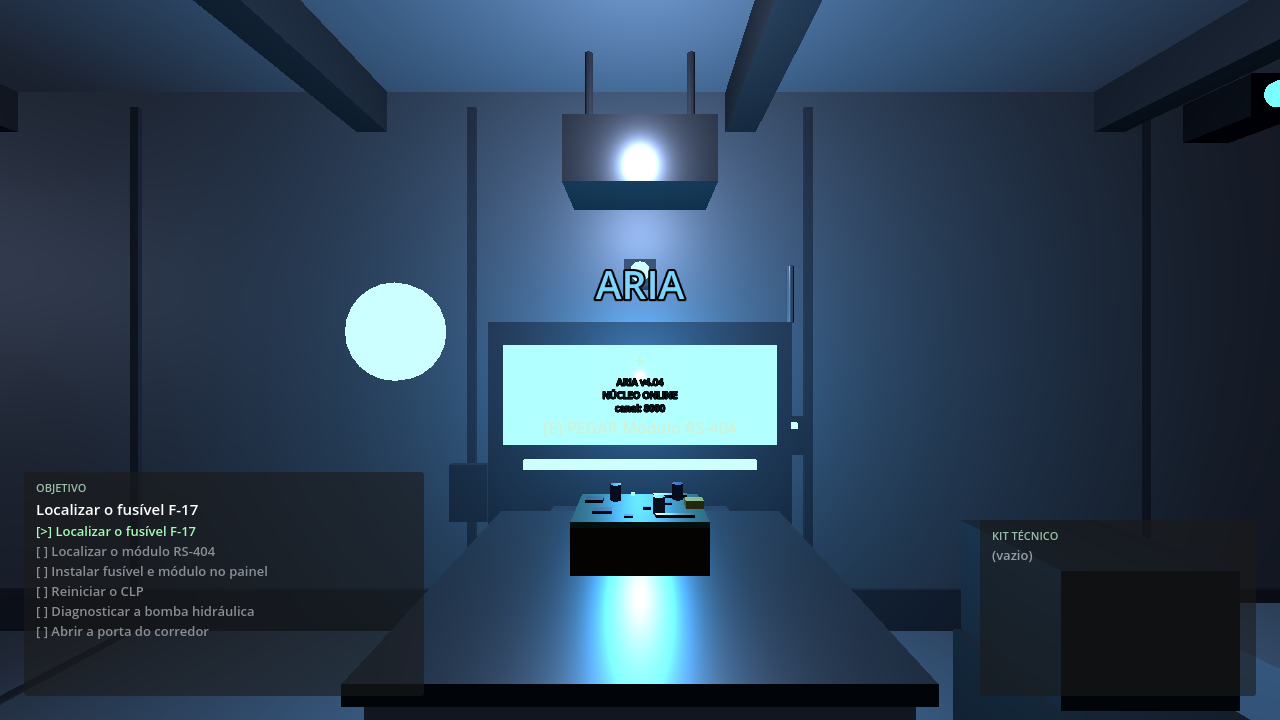
\includegraphics[width=0.72\textwidth]{aria_estacao.png}
\caption{Estação física da \aria{} na sala, com tela de status e ponto de interação.}
\label{fig:aria_estacao}
\end{figure}

\section{\poc{4} --- Mundo reativo}
\label{sec:poc4}

O quarto incremento fez o laboratório reagir ao estado do jogo, com quatro
mecanismos.

\subsection{NPC e diálogo contextual}

Um técnico (NPC) comenta o estado do laboratório --- por exemplo, a situação
da bomba --- de acordo com o momento da missão. O personagem foi modelado como
um corpo único de 882 vértices e 10 materiais (macacão, colete refletivo,
luvas, botas, capacete com lanterna e rosto), com a mesma malha servindo de
colisão; a Figura~\ref{fig:tecnico} mostra o resultado em jogo. A fala do NPC
usa o mesmo canal de mensagens do HUD que os avisos do sistema.

\begin{figure}[htbp]
\centering
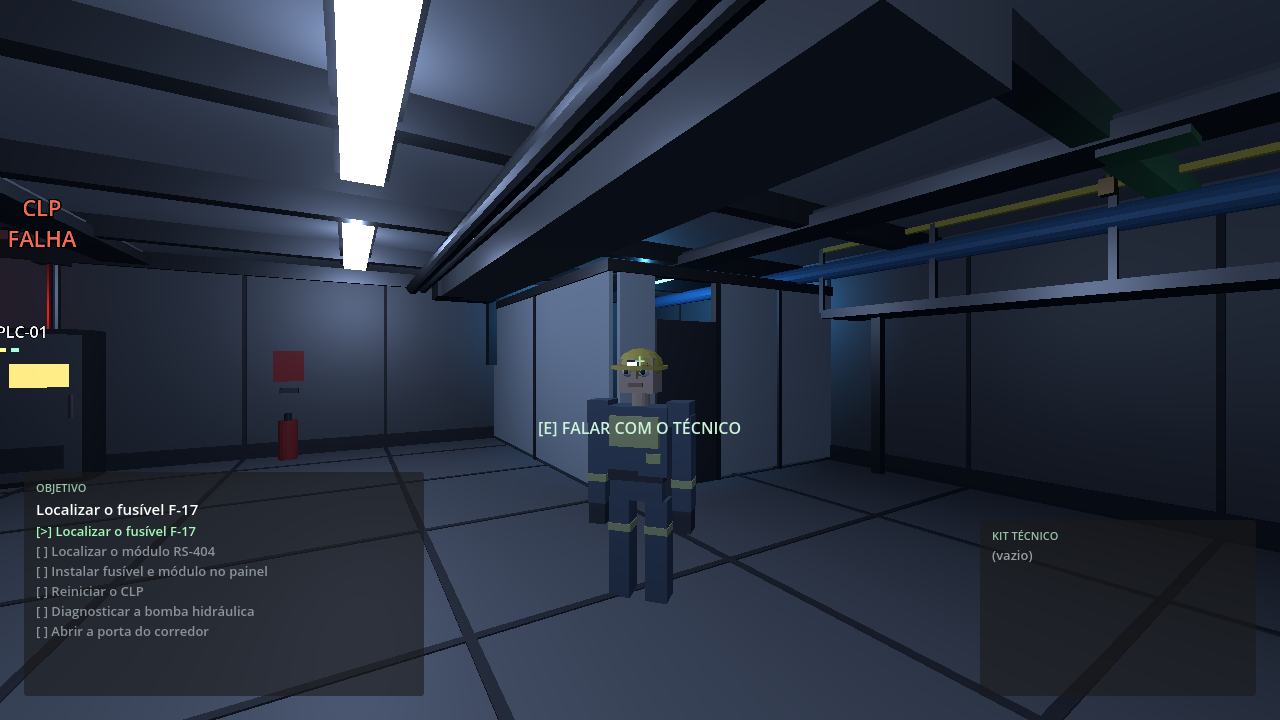
\includegraphics[width=0.72\textwidth]{tecnico.png}
\caption{Técnico (NPC) na sala, com uniforme, capacete e postura de trabalho.}
\label{fig:tecnico}
\end{figure}

\subsection{Memória em camadas}
\label{sec:memoria}

A memória do jogo foi separada em quatro camadas com ciclos de vida
diferentes (Figura~\ref{fig:memoria}): a sessão atual; o estado persistente
(salvo em arquivo); o conhecimento narrativo acumulado (fatos que o jogador
aprendeu sobre a instalação e a IA); e o histórico conversacional. A separação
evita o problema clássico de misturar \emph{flags} de curto prazo com fatos
que precisam sobreviver ao salvamento --- e permite que a IA receba como
contexto exatamente a camada adequada à pergunta.

\begin{figure}[htbp]
\centering
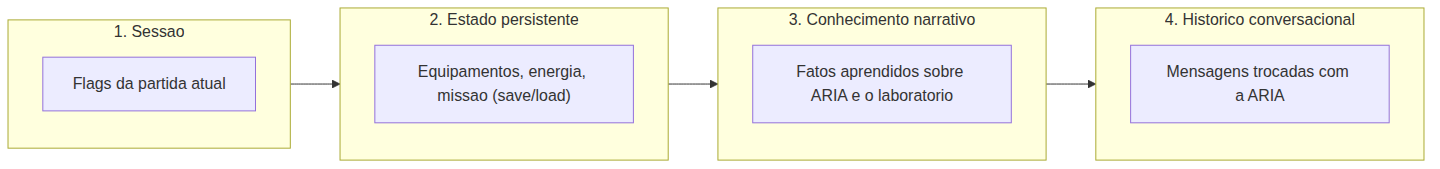
\includegraphics[width=0.95\textwidth]{07_memoria.png}
\caption{As quatro camadas de memória e estado, com ciclos de vida diferentes.}
\label{fig:memoria}
\end{figure}

\subsection{Eventos e iluminação em camadas}

Os eventos do mundo reagem ao estado: luzes mudam conforme a energia, portas
respeitam permissões e o tom da IA muda quando um alerta é ignorado. A
iluminação foi organizada em duas camadas: a luz geral, com dois estados
(claro e emergência), alinhada às luminárias efetivamente visíveis no modelo
3D; e luzes de acento por zona (emergência, IA, painel, bomba, sala de
controle), que preservam a identidade cromática de cada área mesmo no escuro.
Pouco depois de a energia ser restabelecida, uma câmera de segurança da sala
passa a acompanhar o jogador com um movimento limitado --- uma recompensa
visual pelo avanço na missão.

\section{\poc{5} --- Laboratório procedural}
\label{sec:poc5}

O quinto incremento estendeu o jogo para além da sala modelada à mão. Um
gerador cria uma ala de laboratório a partir de módulos tipados (corredor,
controle, bombas, baterias, sensores, arquivo e contenção), cada um com
entradas, saídas, pontos de interesse e iluminação. A geração é determinística
por semente --- a mesma semente produz sempre o mesmo laboratório ---, e a
conectividade é garantida por construção e verificada por busca em largura:
nenhuma sala fica inalcançável (Figura~\ref{fig:gerador}). Essa combinação de
determinismo e garantia de conectividade é o que torna a geração testável
automaticamente, e não apenas plausível.

\begin{figure}[htbp]
\centering
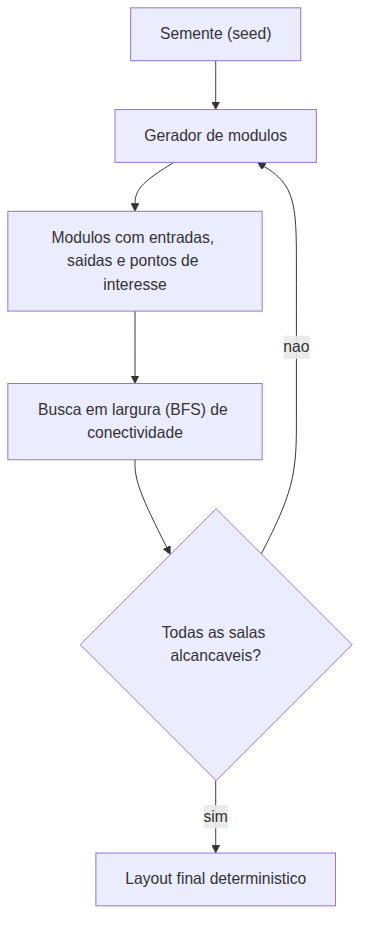
\includegraphics[width=0.72\textwidth]{06_gerador.png}
\caption{Geração procedural: semente, módulos, verificação de conectividade por busca em largura e layout final.}
\label{fig:gerador}
\end{figure}

\section{\poc{6} --- Recorte vertical}
\label{sec:poc6}

O sexto incremento fechou o arco jogável: tutorial, persistência, áudio e
epílogo.

\subsection{Tutorial e progressão}

O jogo começa com um tutorial de controles apresentado em etapas curtas, que
apresenta ao jogador a movimentação, a câmera e a interação antes que a
missão exija qualquer procedimento. A estrutura dramática em quatro atos
(Figura~\ref{fig:narrativa}) conduz a ficção: a falha inicial, a percepção de
que há algo inconsistente, a revelação sobre a IA e a escolha final.

\begin{figure}[htbp]
\centering
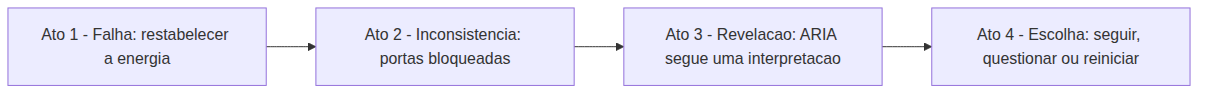
\includegraphics[width=0.95\textwidth]{09_narrativa.png}
\caption{Estrutura dramática em quatro atos, do restabelecimento da energia à escolha final.}
\label{fig:narrativa}
\end{figure}

\subsection{Persistência}

O progresso é salvo em arquivo local e restaurado com fidelidade: o
salvamento inclui o ponto da missão, as \emph{flags} de estado, os estados
dos equipamentos e o conhecimento narrativo acumulado. Após o carregamento, o
mundo é reconciliado --- luzes, portas e equipamentos refletem o estado
restaurado ---, o que é verificado automaticamente.

\subsection{Áudio}

Os efeitos sonoros são originais, gerados por um script do próprio projeto:
coleta, instalação, porta, erro, alarme, interface e ambiência. A ambiência é
um laço contínuo de baixa intensidade, e os efeitos pontuais usam um conjunto
de canais reutilizáveis. Um defeito encontrado e corrigido nesse subsistema
merece registro: como os arquivos de áudio são importados pelo motor em
formato comprimido, o cálculo do ponto de repetição do laço precisava usar a
duração real do arquivo, e não o tamanho do bloco de dados comprimido --- erro
que causava um laço de menos de um segundo em um trecho de quatro segundos. A
correção foi acompanhada de uma verificação de regressão na suíte.

\subsection{Epílogo}

Ao final, o jogador escolhe entre seguir as instruções da IA, questioná-la ou
reiniciar seu núcleo. A escolha é registrada no estado persistente e altera o
texto final exibido. A decisão de projeto --- declarada no escopo do trabalho
--- foi manter a ramificação restrita ao epílogo, em vez de multiplicar
caminhos.

\section{Engenharia de desempenho}
\label{sec:desempenho_dev}

O alvo de execução em computador sem GPU dedicada guiou decisões em todas as
etapas. No motor, adotou-se o renderizador compatível
(\texttt{gl\_compatibility}), geometria simples, número controlado de luzes e
ausência de efeitos de pós-processamento custosos. No asset, o emissivo foi
dosado (luzes de ambiente em intensidade 1,5--1,6; telas em 1,1--1,3) para
não estourar em branco na ausência de \emph{bloom}. No detalhamento, os
efeitos de animação que o formato glTF não suporta (emissão intermitente)
foram convertidos em lógica de script de baixo custo. E a iluminação do nível
segue as posições das luminárias efetivamente modeladas --- a luz nasce onde
o jogador vê a fonte ---, o que evita tanto o gasto desnecessário quanto o
resultado visual incoerente.

O orçamento de tempo por quadro a 60 Hz é de
\begin{equation}
\label{eq:orcamento}
t_{\text{quadro}} = \frac{1}{f} = \frac{1}{60} \approx 16{,}67\ \text{ms},
\end{equation}
\noindent e foi esse orçamento --- considerando lógica de \emph{gameplay},
física simplificada, iluminação em camadas e interface --- que orientou duas
decisões estruturais: manter efeitos de pós-processamento fora do projeto e
converter animações de material em lógica de script barata. A iluminação em
camadas é um compromisso explícito: em vez de muitas luzes dinâmicas com
sombras (custo alto em GPU integrada), usa-se um conjunto reduzido de luzes
sem sombras, compensado por emissivos dosados no asset e por cores de acento
por zona.

\section{Interface e direção visual}
\label{sec:interface}

A interface do jogo foi tratada como instrumento, não como menu genérico de
videogame. O HUD mantém, no canto superior, o relógio da instalação, a
identificação do setor e o estado de energia; abaixo, à esquerda, a lista de
objetivos com marcação de passo concluído --- o mesmo encadeamento da missão
descrita na \autoref{sec:interacao}; e, na base, os convites de interação e de
status. O resultado é um painel que informa sem competir com o cenário.

O terminal da IA recebeu tratamento visual próprio, com cabeçalho de
identificação do núcleo, histórico de mensagens e linha de entrada. A escolha
de exibir a conversa como terminal --- em vez de balões de diálogo --- reforça
a ficção de sistema operacional e acomoda naturalmente a latência da IA:
enquanto a resposta não chega, o cursor permanece ativo, sem quebrar a
imersão.

O inventário também é diegético: em vez de uma grade abstrata, o jogador vê
o kit técnico com seus itens (fusível, módulo e chave), em uma lista curta que
reforça a correspondência entre o que se carrega e o que se instala nos
painéis. A paleta geral é escura, com cores de função --- branco para
iluminação geral, ciano para interfaces da IA, âmbar para máquinas e vermelho
para emergência e travamentos ---, mantendo coerência com a iluminação em
camadas descrita na \autoref{sec:poc4}.

\section{Level design do recorte vertical}
\label{sec:level_design}

O recorte vertical organiza o espaço em torno de um corredor central
(Figura~\ref{fig:mapa}). A sala principal --- onde começa o jogo --- concentra
a bancada, o painel, o CLP, a bomba e a estação da IA; as demais salas são
alcançadas pelo corredor, que funciona como rota principal e como ponto de
orientação. Os pontos de interesse (arquivo, energia, bombas e controle)
ficam nas extremidades, e o percurso final conduz ao núcleo da IA.

\begin{figure}[htbp]
\centering
\begin{tikzpicture}[font=\scriptsize,
  sala/.style={draw, rounded corners=2pt, align=center, inner sep=3pt,
               minimum width=2.5cm, minimum height=0.95cm, fill=black!4},
  seta/.style={-{Stealth[length=1.8mm]}, semithick}]
\node[sala] (cor) {Corredor\\(rota principal)};
\node[sala, left=14mm of cor] (bom) {Bombas (PI)};
\node[sala, right=14mm of cor] (ctl) {Controle --- IA (PI)};
\node[sala, above=10mm of cor] (arq) {Arquivo (PI)};
\node[sala, below=10mm of cor] (ene) {Energia (PI)};
\draw[seta] (bom) -- (cor);
\draw[seta] (cor) -- (ctl);
\draw[seta] (cor) -- (arq);
\draw[seta] (cor) -- (ene);
\draw[seta] (ene) -- (ctl);
\end{tikzpicture}
\caption{Organização espacial do recorte vertical: corredor central, pontos de interesse (PI) nas extremidades e percurso final até o núcleo da IA.}
\label{fig:mapa}
\par\vspace{2pt}{\footnotesize Fonte: elaborado pelo autor (2026), a partir do level design do projeto.}
\end{figure}

Três princípios guiaram o traçado: o jogador deve sempre saber onde está
(landmarks visuais, letreiros e iluminação por zona); deve saber qual é o
objetivo corrente (HUD persistente); e deve reconhecer a interação possível
(convite contextual). O que o jogo deliberadamente \emph{não} entrega de
imediato é a motivação da IA --- a ambiguidade é conteúdo narrativo, não
falha de comunicação.

\section{Persistência: estrutura do salvamento}
\label{sec:persistencia}

O salvamento é um arquivo de texto no diretório do usuário, com estrutura
versionada em campos independentes (Quadro~\ref{quad:save}). A separação
segue as camadas de memória descritas na \autoref{sec:memoria}: o que é
estado persistente entra no arquivo; o que é sessão não entra. O carregamento
reconcilia o mundo --- luzes, portas e equipamentos assumem o estado salvo
---, e essa reconciliação é verificada automaticamente pelo teste da etapa
correspondente.

\begin{quadro}[htbp]
\centering
\caption{Estrutura do arquivo de salvamento (campos principais).}
\label{quad:save}
\begin{verbatim}
{
  "versao": 1,
  "missao": {"passo_atual": 5, "concluida": true},
  "flags": {"energia_restaurada": true, ...},
  "equipamentos": {"bomba": "RUNNING", "clp": "RUNNING", ...},
  "memoria_narrativa": ["bomba", "revelacao", ...],
  "epilogo": "questionar"
}
\end{verbatim}
\par\vspace{2pt}{\footnotesize Fonte: elaborado pelo autor (2026), a partir do sistema de salvamento do projeto.}
\end{quadro}

\section{Generação procedural: algoritmo}
\label{sec:algoritmo_gerador}

O gerador da ala procedural trabalha em duas fases (Quadro~\ref{quad:gerador}):
primeiro constrói uma árvore de expansão a partir da semente, ligando módulos
por portas compatíveis; em seguida, verifica por busca em largura que todos os
módulos são alcançáveis a partir da entrada e que os pontos de interesse
estão em regiões acessíveis. Se a verificação falha, o gerador descarta o
layout e tenta de novo --- com a mesma semente, o resultado é sempre o mesmo,
o que torna a geração testável e os defeitos reproduzíveis.

\begin{quadro}[htbp]
\centering
\caption{Pseudocódigo do gerador procedural (duas fases).}
\label{quad:gerador}
\begin{verbatim}
gerar(seed):
    rng = aleatorio(seed)
    arvore = expandir_modulos(rng)      # portas compativeis
    layout = posicionar(arvore)
    enquanto nao conectado(layout):
        layout = tentar_novamente(rng)  # rng preserva o determinismo
    retornar layout
\end{verbatim}
\par\vspace{2pt}{\footnotesize Fonte: elaborado pelo autor (2026), a partir do gerador do projeto.}
\end{quadro}

\section{Operação: execução, registros e encerramento}
\label{sec:operacao}

O projeto oferece dois scripts de operação: um para iniciar o jogo (e,
quando disponível, o serviço de IA) e outro para encerrar ambos com segurança.
Os registros de execução e os identificadores de processo ficam em um
diretório de trabalho; ao encerrar, o script pede a saída por um arquivo-sinal
que o próprio jogo observa, em vez de enviar sinais do sistema operacional.
Essa decisão --- incomum, mas necessária --- responde a uma restrição do
ambiente: o motor instalado por pacote confinado recusa sinais externos, de
modo que tanto o encerramento assistido quanto a própria suíte de testes
dependem do canal cooperativo. O detalhe é registrado aqui porque afeta
diretamente a reprodutibilidade das execuções.

\section{Subsistema de áudio}
\label{sec:audio_dev}

O áudio é inteiramente original e gerado por um script do projeto, sem
conteúdo de terceiros: sete efeitos que cobrem coleta, instalação, porta,
erro, alarme, interface e ambiência (Quadro~\ref{quad:audio}). A ambiência é
um laço contínuo de baixa intensidade, e os efeitos pontuais compartilham um
conjunto de canais reutilizáveis, evitando sobreposições quando o jogador
interage rapidamente.

\begin{quadro}[htbp]
\centering
\caption{Catálogo de sons do jogo (gerados por script próprio).}
\label{quad:audio}
\footnotesize
\begin{tabular}{@{}>{\raggedright\arraybackslash}p{2.2cm} >{\raggedright\arraybackslash}p{5.4cm} >{\raggedright\arraybackslash}p{5.2cm}@{}}
\toprule
Som & Uso & Característica \\
\midrule
\texttt{pickup} & coleta de item & curto, ascendente \\
\texttt{install} & instalação no painel & curto, mecânico \\
\texttt{door} & abertura da porta & ruído descendente \\
\texttt{error} & ação inválida & tom descendente seco \\
\texttt{alarm} & alerta do sistema & pulsado, mais longo \\
\texttt{ui} & interface e terminal & clique discreto \\
\texttt{hum} & ambiência contínua & laço de baixa frequência \\
\bottomrule
\end{tabular}
\par\vspace{2pt}{\footnotesize Fonte: elaborado pelo autor (2026), a partir do gerador de áudio do projeto.}
\end{quadro}

\section{Considerações do capítulo}
\label{sec:consideracoes_desenvolvimento}

O desenvolvimento seguiu uma trajetória de complexidade crescente: entrada e
movimento; asset e interação; IA com fronteira de segurança; mundo reativo;
geração procedural; e fechamento narrativo. Cada etapa preservou a
possibilidade de executar e demonstrar o jogo completo, o que permitiu que as
evidências fossem coletadas continuamente --- e não apenas ao final. Os
resultados quantitativos dessa construção são apresentados no
\autoref{cap:resultados}.

\chapter{Experimentos e resultados}
\label{cap:resultados}

Este capítulo apresenta os resultados obtidos com os procedimentos descritos
no \autoref{cap:metodos}, na máquina de referência
(Tabela~\ref{tab:ambiente}), na execução de referência de 10 de setembro de
2026. Todos os números são oriundos de execução real e podem ser reproduzidos
pelos comandos descritos no \autoref{ap:repositorio}.

\section{Verificação funcional automatizada}
\label{sec:res_testes}

A suíte automatizada cobre as seis etapas do desenvolvimento e o adaptador de
IA. A Tabela~\ref{tab:testes} detalha a distribuição das verificações por
etapa; a Figura~\ref{fig:verificacoes} apresenta a mesma informação
visualmente. No total, foram executadas \textbf{211 verificações do motor e 16
testes do adaptador, todas aprovadas}, sem falhas.

% Verificações automatizadas por etapa (capítulo 6).
\begin{table}[htbp]
\centering
\caption{Verificações automatizadas por etapa do projeto (execução de referência de 2026-09-10).}
\label{tab:testes}
\footnotesize
\begin{tabular}{@{}>{\raggedright\arraybackslash}p{1.6cm} >{\raggedright\arraybackslash}p{8.4cm} >{\centering\arraybackslash}p{2.2cm}@{}}
\toprule
Etapa & Escopo validado & Verificações \\
\midrule
\poc{1} & Fundação jogável: entrada semântica, movimento, colisão, câmera, pausa, HUD e diagnóstico de entrada & 77 \\
\poc{2} & Laboratório funcional: interação, inventário, porta, missão, identidade visual da sala & 34 \\
\poc{3} & IA: adaptador, terminal, limites de tempo, validação de intenção e \emph{fallback} & 25--26 \\
\poc{4} & Mundo reativo: NPC, luzes por energia, câmera de segurança, tom da IA e memória em camadas & 21 \\
\poc{5} & Laboratório procedural: determinismo por semente e conectividade entre módulos & 23 \\
\poc{6} & Recorte vertical: tutorial, missão completa, persistência, áudio e epílogo & 30 \\
Adaptador & API de IA (Python): contratos, validação, erros e limites & 16 \\
\midrule
\textbf{Total} & & \textbf{211 + 16} \\
\bottomrule
\end{tabular}
\par\vspace{2pt}{\footnotesize Fonte: elaborado pelo autor (2026), a partir da execução de \texttt{tests/run\_all.sh}. A etapa \poc{3} vale 25 com o adaptador no ar e 26 com o adaptador desligado.}
\end{table}


\begin{figure}[htbp]
\centering
\begin{tikzpicture}
\begin{axis}[
  ybar,
  width=0.9\textwidth,
  height=5.6cm,
  bar width=10pt,
  ymin=0,
  ylabel={verificações},
  symbolic x coords={POC1,POC2,POC3,POC4,POC5,POC6,Adaptador},
  xtick=data,
  nodes near coords,
  every node near coord/.append style={font=\scriptsize},
  tick label style={font=\small},
  label style={font=\small},
]
\addplot[fill=black!35] coordinates {
  (POC1,77) (POC2,34) (POC3,26) (POC4,21) (POC5,23) (POC6,30) (Adaptador,16)
};
\end{axis}
\end{tikzpicture}
\caption{Distribuição das verificações automatizadas por etapa do projeto, incluindo os testes do adaptador de IA.}
\label{fig:verificacoes}
\par\vspace{2pt}{\footnotesize Fonte: elaborado pelo autor (2026), a partir da execução da suíte.}
\end{figure}

Dois comentários sobre a leitura da tabela. Primeiro, a etapa \poc{3} varia
entre 25 e 26 verificações: com o adaptador no ar, um dos casos de
\emph{fallback} dá lugar à validação da resposta real do modelo, de modo que
o número depende do contexto de execução. Segundo, o tamanho da suíte não é
uniforme entre etapas --- a fundação jogável concentra 77 verificações porque
precisou cobrir movimento, colisão, câmera, entrada e interface.

\section{Critérios de aceitação}
\label{sec:res_criterios}

A Tabela~\ref{tab:aceitacao_resumo} resume o status dos critérios de
aceitação. Treze dos quatorze itens verificáveis são cobertos por testes
automatizados; os pontos de contato físico (mouse capturado e joystick real)
e o percurso completo por uma pessoa permanecem como validação manual
declarada. O requisito de empacotamento (FR-033) segue aberto: a geração do
executável dependia de modelos de exportação do motor ausentes no ambiente.

% Status dos critérios de aceitação (capítulo 6).
\begin{table}[htbp]
\centering
\caption{Status dos critérios de aceitação e requisito de empacotamento.}
\label{tab:aceitacao_resumo}
\footnotesize
\begin{tabular}{@{}>{\raggedright\arraybackslash}p{1.5cm} >{\raggedright\arraybackslash}p{8.0cm} >{\raggedright\arraybackslash}p{2.6cm}@{}}
\toprule
Critério & Verificação & Status \\
\midrule
CA-001 & Movimento por ação semântica, colisão e piso & Aprovado (automatizado) \\
CA-002 & Rotação de câmera por ação; limites de inclinação & Parcial (mouse = manual) \\
CA-003 & Pausa e retomada com menu & Aprovado (automatizado) \\
CA-004 & Zona morta configurável e tratamento de \emph{hotplug} & Parcial (joystick físico = manual) \\
CA-005 & Carga do jogo sem assets externos obrigatórios & Aprovado (automatizado) \\
CA-006 & Convite contextual e interação por proximidade & Aprovado (automatizado) \\
CA-007 & Coleta, instalação no painel e avanço da missão no HUD & Aprovado (automatizado) \\
CA-008 & Estados de equipamento serializáveis (desligado, falha, pronto, operando) & Aprovado (automatizado) \\
CA-009 & \emph{Fallback} com o serviço de IA indisponível, sem travar & Aprovado (automatizado) \\
CA-010 & Intenção fora do conjunto permitido convertida para \texttt{NONE} & Aprovado (automatizado) \\
CA-011 & Mundo reage a eventos (NPC, luzes, tom da IA) & Aprovado (automatizado) \\
CA-012 & Mesma semente produz o mesmo layout; salas alcançáveis & Aprovado (automatizado, 6 sementes) \\
CA-013 & Jogo completo do início ao fim & Parcial (percurso humano = manual) \\
FR-033 & Geração de executável independente & Aberto (modelos de exportação ausentes no ambiente) \\
\bottomrule
\end{tabular}
\par\vspace{2pt}{\footnotesize Fonte: elaborado pelo autor (2026), a partir da especificação e da execução da suíte.}
\end{table}


\section{Desempenho gráfico}
\label{sec:res_desempenho}

A cena completa --- com a sala detalhada, o NPC, as camadas de iluminação e
os letreiros --- executou a \textbf{60 quadros por segundo}, limitados por
sincronismo vertical, em resolução de 1280$\times$720, na GPU integrada AMD
Radeon Graphics. O valor foi mantido após o detalhamento final da sala (342
nós e 37 materiais no asset), dentro do critério NFR-001. A
Figura~\ref{fig:sala_energizada} mostra a cena com a energia restabelecida ---
o estado em que sensores, luzes e câmera de segurança estão todos ativos, ou
seja, o cenário mais carregado do jogo.

\begin{figure}[htbp]
\centering
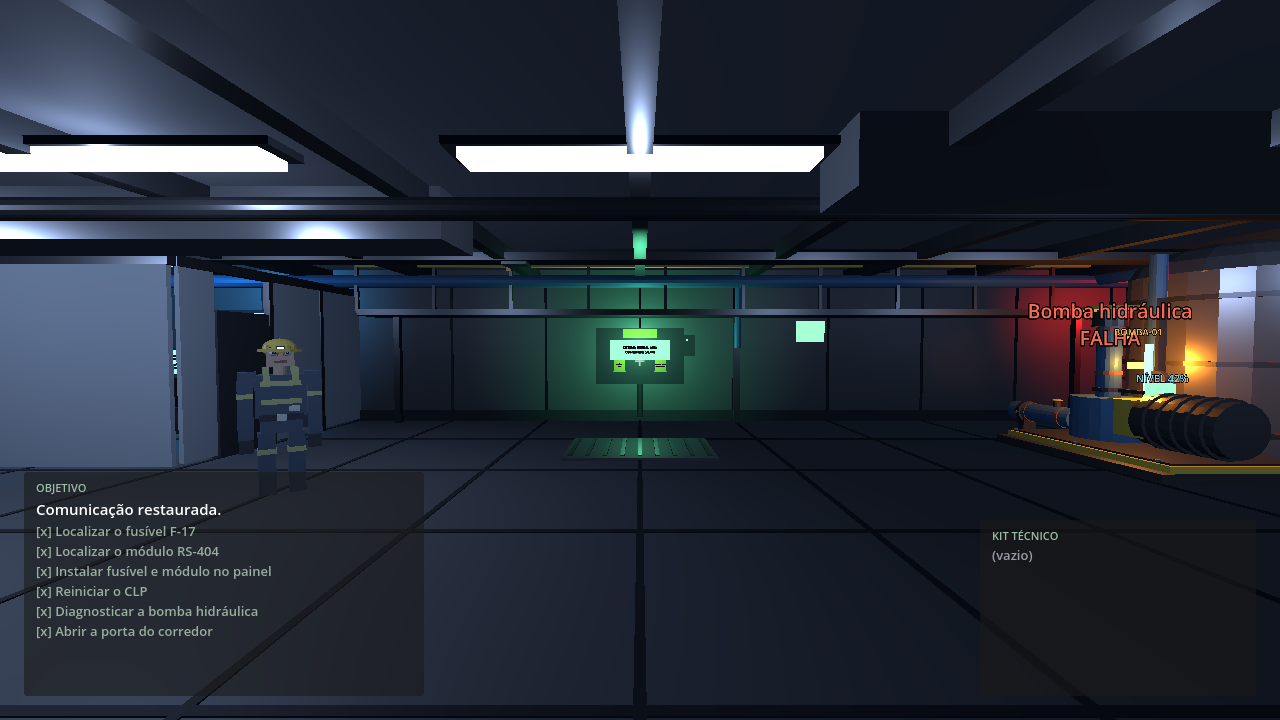
\includegraphics[width=0.8\textwidth]{sala_energizada.png}
\caption{Sala com a energia restaurada: luminárias do teto acesas, câmera de segurança ativa, porta B1 liberada e letreiros das estações. Captura em 1280$\times$720.}
\label{fig:sala_energizada}
\end{figure}

Duas ressalvas tornam a leitura honesta. A primeira: o valor de 60 quadros
por segundo é um limite imposto pelo sincronismo vertical, não uma medida de
folga do sistema; sem sincronismo, a taxa observada seria maior, mas o
trabalho não mediu esses valores. A segunda: não foram coletadas métricas de
tempo de quadro por percentil (por exemplo, o quadro mais lento de cada
segundo), que seriam necessárias para caracterizar engasgos transitórios
[MEDIÇÃO DE FRAME TIME NÃO REALIZADA]. Ambas as lacunas estão registradas
como trabalhos futuros.

\section{Complexidade do asset 3D}
\label{sec:res_asset}

A inspeção programática do arquivo exportado mediu: 342 nós, 37 materiais,
35 nós de colisão embutidos e tamanho final de 1.018,7~KB. Esses números
delimitam o orçamento de complexidade do cenário e explicam, em parte, o
desempenho obtido: o detalhamento foi feito com geometria econômica e
materiais reutilizados, e as animações que o formato não suporta (emissão
intermitente) foram convertidas em lógica de script.

\section{Latência da conversa com a IA}
\label{sec:res_latencia}

A Tabela~\ref{tab:latencia} apresenta as três medições de latência
realizadas com o modelo local \texttt{llama3.1:8b}. O pior caso (22,0~s) foi
a chamada direta ao adaptador em partida fria, quando o modelo precisa ser
carregado na memória; no uso cotidiano pelo terminal do jogo, a resposta
levou 16,1~s; e no teste ao vivo do cliente, 12,9~s, com aprovação integral
das verificações de integração.

% Latências medidas (capítulo 6).
\begin{table}[htbp]
\centering
\caption{Latências medidas da conversa com a IA local (\texttt{llama3.1:8b}) em três contextos independentes.}
\label{tab:latencia}
\footnotesize
\begin{tabular}{@{}>{\raggedright\arraybackslash}p{5.4cm} l r >{\raggedright\arraybackslash}p{3.4cm}@{}}
\toprule
Contexto & Intenção & Latência & Observação \\
\midrule
Chamada direta ao adaptador (partida fria) & DIAGNOSE & 22,0 s & confiança 0,9 \\
Terminal no jogo (uso normal) & STATUS & 16,1 s & evidência visual capturada \\
Cliente no jogo (teste ao vivo) & HINT & 12,9 s & 5 de 5 verificações \\
\bottomrule
\end{tabular}
\par\vspace{2pt}{\footnotesize Fonte: elaborado pelo autor (2026). Uma execução por contexto; valores indicativos, não estatísticos.}
\end{table}


A Figura~\ref{fig:terminal_evidencia} registra a evidência visual do
contexto em jogo: a pergunta do jogador e a resposta do modelo, exibidas no
terminal da \aria{}. A Figura~\ref{fig:tela_evidencia} mostra a tela de status
da estação no mundo 3D, que dá coerência diegética ao subsistema.

\begin{figure}[htbp]
\centering
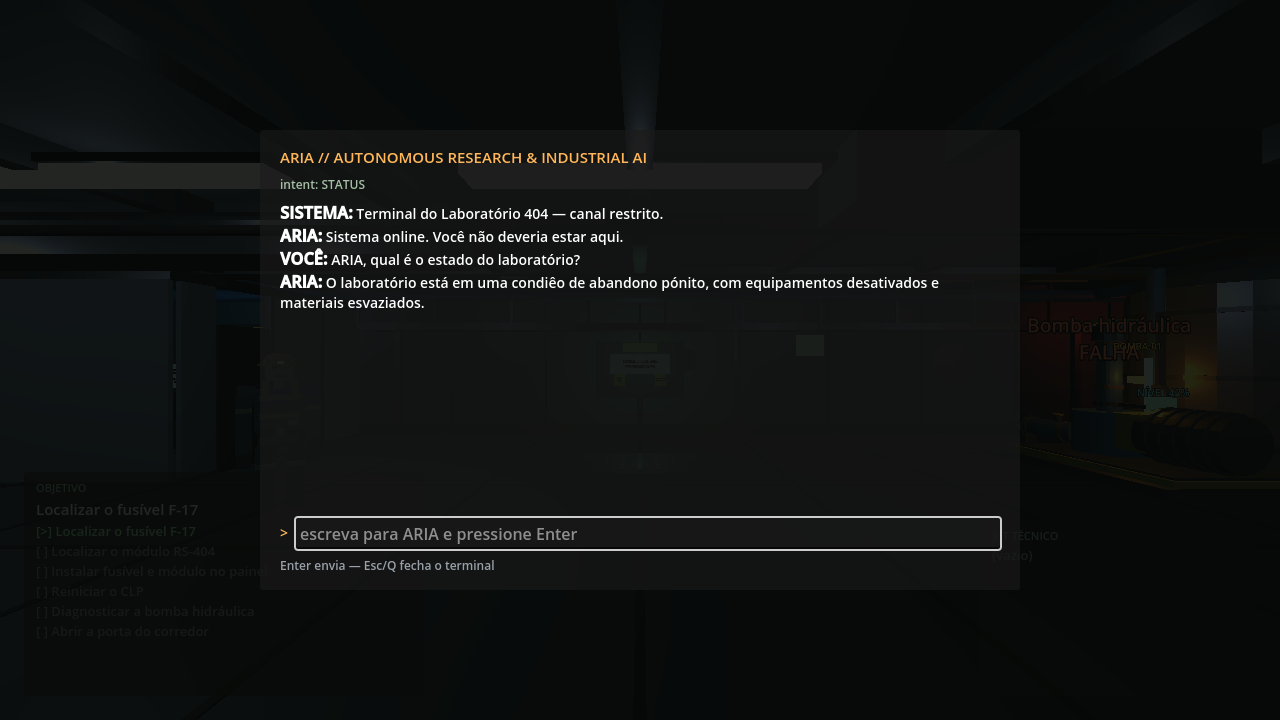
\includegraphics[width=0.8\textwidth]{terminal_aria.png}
\caption{Terminal da \aria{} no jogo com a resposta do modelo local (latência de 16,1~s, intenção \texttt{STATUS}).}
\label{fig:terminal_evidencia}
\end{figure}

\begin{figure}[htbp]
\centering
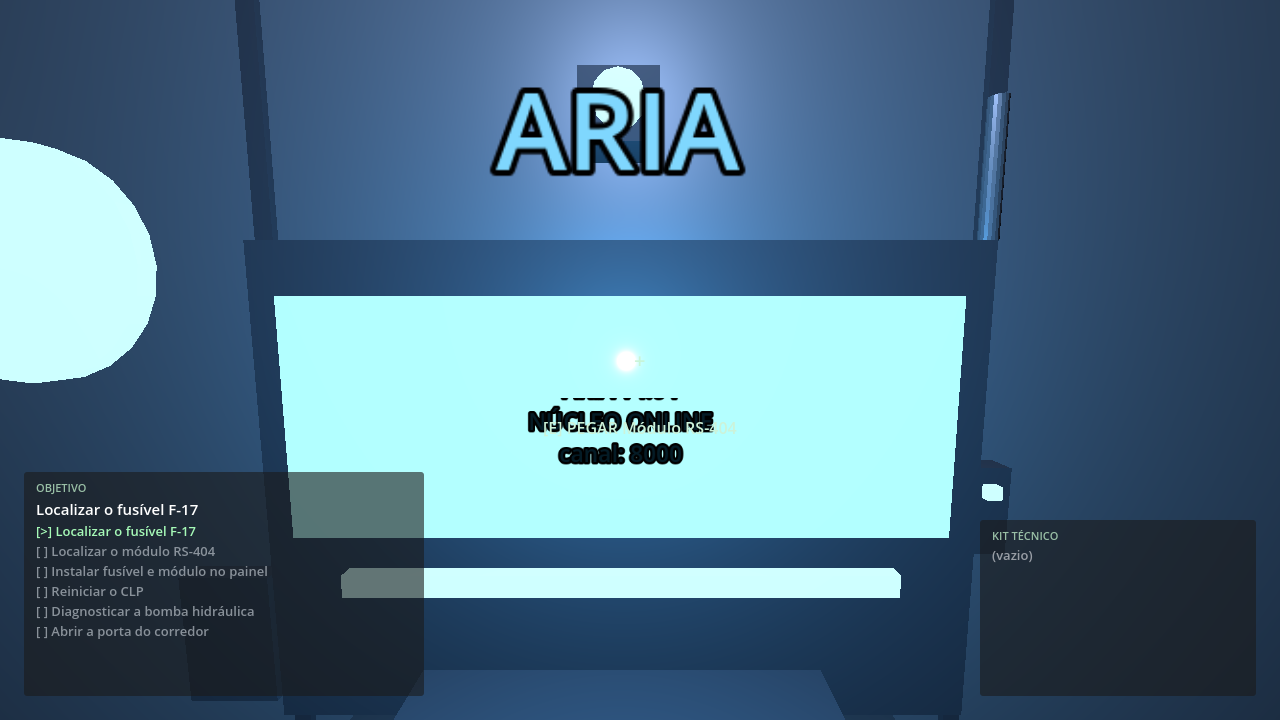
\includegraphics[width=0.8\textwidth]{tela_aria.png}
\caption{Tela de status da estação da IA no mundo 3D, com identificação do núcleo e do canal de comunicação.}
\label{fig:tela_evidencia}
\end{figure}

Três observações qualificam esses números. Primeiro, as medições foram feitas
com um modelo \emph{maior} do que o alvo declarado no projeto
(\texttt{llama3.2:3b}, não instalado no ambiente): espera-se que o modelo-alvo
seja mais rápido, mas isso não foi medido [MODELO-ALVO NÃO EXECUTADO].
Segundo, cada contexto foi medido em uma execução; os valores são
indicativos, não estatísticos. Terceiro, o comportamento de segurança foi
verificado independentemente das medições de velocidade: com o serviço fora
do ar, o jogo respondeu com texto de \emph{fallback} e intenção \texttt{NONE},
sem travar --- resultado coberto pelos testes automatizados do adaptador e do
cliente.

\section{Evidências visuais e demonstração}
\label{sec:res_evidencias}

Além das figuras deste capítulo, o projeto mantém um conjunto de evidências
visuais produzido por um arnês de captura que posiciona o jogador em pontos
pré-determinados, podendo inclusive concluir a missão para registrar o estado
final (a Figura~\ref{fig:sala_energizada} foi gerada nesse modo). Um vídeo de
demonstração de 1~min~08~s percorre a missão do segundo incremento, do painel
à abertura da porta \cite{lab404video}. Código, especificação, capturas e
vídeo estão publicamente disponíveis \cite{lab404repo}.

\section{Reprodutibilidade dos resultados}
\label{sec:reprodutibilidade}

Todos os resultados deste capítulo são reproduzíveis a partir do repositório
público \cite{lab404repo} com os comandos a seguir; na primeira execução, o
projeto importa os recursos (modelo 3D e áudio), e nas seguintes os comandos
abaixo bastam.

\begin{itemize}
  \item \texttt{tests/run\_all.sh} --- executa a suíte completa e imprime, por
  etapa, o número de verificações e de falhas (esperado: todas aprovadas);
  \item \texttt{godot4 --path .} ou \texttt{./start.sh} --- inicia o jogo (o
  segundo inicia também o serviço de IA, quando o ambiente Python existe);
  \item \texttt{.venv/bin/uvicorn scripts.aria\_adapter:app --port 8000} ---
  inicia o serviço de IA, com o modelo local servido pelo Ollama;
  \item cena de captura com variáveis de pose e de conclusão da missão ---
  reproduz as imagens de evidência deste capítulo;
  \item script de inspeção do arquivo GLB --- reproduz as contagens de nós,
  materiais e colisões.
\end{itemize}

Variações de hardware, de versão de biblioteca e de modelo de linguagem
alteram os valores de desempenho e de latência, mas não os resultados
funcionais: a suíte é determinística no que verifica, e a geração procedural
é determinística por semente.

\section{Matriz de evidências}
\label{sec:res_matriz}

O Quadro~\ref{quad:matriz} resume a correspondência entre as afirmações
quantitativas do trabalho e as evidências que as sustentam --- a versão
completa está no arquivo de rastreabilidade do projeto.

\begin{quadro}[htbp]
\centering
\caption{Correspondência entre afirmações quantitativas e evidências.}
\label{quad:matriz}
\footnotesize
\begin{tabular}{@{}>{\raggedright\arraybackslash}p{4.6cm} >{\raggedright\arraybackslash}p{4.4cm} >{\raggedright\arraybackslash}p{3.8cm}@{}}
\toprule
Afirmação & Evidência & Fonte \\
\midrule
211 verificações do motor + 16 testes do adaptador aprovados & Execução da suíte completa & \texttt{tests/run\_all.sh}; cenas de teste e suíte Python \\
60 FPS (vsync) em 1280$\times$720 na GPU integrada & Leitura do motor em execução na cena completa & Execução na máquina de referência (Tabela~\ref{tab:ambiente}) \\
Latências de 12,9 s a 22,0 s & Três execuções cronometradas & Relatório de execução e captura do terminal \\
342 nós, 37 materiais, 35 colisões, 1.018,7 KB & Inspeção programática do GLB & \texttt{assets/lab404/}\allowbreak\texttt{lab\_sala\_poc2.glb} \\
Missão completa do início ao fim (automatizado) & Cena de teste da etapa final & \texttt{tests/poc6\_test.gd} \\
Degradação segura da IA sob falha & Testes de contrato e de integração & CA-009 e CA-010 (suíte do adaptador) \\
\bottomrule
\end{tabular}
\par\vspace{2pt}{\footnotesize Fonte: elaborado pelo autor (2026).}
\end{quadro}

\section{Síntese dos resultados}
\label{sec:res_sintese}

Em síntese, os experimentos demonstram: (i) o sistema é funcionalmente
verificável --- 227 verificações automatizadas no total, todas aprovadas;
(ii) o desempenho atende ao critério de hardware modesto no cenário mais
carregado; (iii) a integração com a IA local funciona de ponta a ponta, com
latências de 12,9~s a 22,0~s e degradação segura garantida; e (iv) o
artefato 3D permanece dentro de um orçamento de complexidade compatível com
GPU integrada. As limitações desses resultados --- e o que elas implicam ---
são discutidas no capítulo seguinte.

\chapter{Discussão}
\label{cap:discussao}

\section{Respostas às questões de pesquisa}
\label{sec:respostas}

\textbf{RQ1 --- integração segura.} A arquitetura adotada --- IA em processo
separado, contrato de dados validado, intenções restritas e sanitização em
duas camadas independentes --- mostrou-se suficiente para que a IA
participasse da ficção (conversa, comentários sobre o estado do mundo, tom
variável) sem receber qualquer capacidade de alterar o jogo. Em todos os
cenários de falha exercitados pelos testes --- serviço fora do ar, resposta
inválida, modelo lento, JSON malformado, intenção desconhecida --- o pior
resultado observado foi uma resposta de \emph{fallback}: nunca um travamento,
nunca um comando executado.

\textbf{RQ2 --- viabilidade em hardware modesto.} O jogo manteve 60 quadros
por segundo (limitados por sincronismo vertical) em 1280$\times$720 na GPU
integrada, com o cenário final completo, e a conversa local respondeu entre
12,9~s e 22,0~s com um modelo de 8 bilhões de parâmetros. Essa ordem de
grandeza é adequada à interação conversacional por turnos --- o formato
adotado no jogo --- e inadequada a reações em tempo real, o que reforça a
decisão de manter a IA fora do laço de controle.

\textbf{RQ3 --- rastreabilidade.} A combinação de especificação prévia,
critérios de aceitação verificáveis e suíte automatizada permitiu conduzir um
desenvolvimento de autor único, com apoio de agentes de IA, mantendo cada
afirmação do projeto atrelada a um teste ou a uma medição. As seis etapas
fecharam com a suíte verde, e as pendências reais do protótipo (validação
manual, empacotamento, modelo-alvo) estão declaradas --- não maquiadas.

\section{Interpretação dos resultados}
\label{sec:interpretacao}

Três leituras merecem destaque. A primeira é que o valor educacional do
artefato não foi medido: o que este trabalho demonstra é a viabilidade
técnica de um instrutor ficcional sempre disponível, com custo de
infraestrutura zero (nenhum serviço pago, nenhuma chave de API) e degradação
segura. A segunda é que a latência de segundos molda o \emph{design} do
diálogo: perguntas e respostas funcionam bem; reações instantâneas, não. A
terceira é que o detalhamento visual tem custo gerenciável quando segue
convenções (escala, nomenclatura, colisão embutida): o cenário cresceu sem
comprometer o desempenho.

\section{Comparação com a literatura}
\label{sec:comparacao}

A comparação com os trabalhos relacionados é qualitativa, conforme declarado
no \autoref{cap:relacionados} e sintetizado no Quadro~\ref{quad:comparativo}.
O contraste central é de propósito: \emph{Generative Agents}
\cite{park2023generative} e \emph{Voyager} \cite{wang2023voyager} investigam o
que a autonomia produz; o Laboratório 404 investiga o que se preserva quando
a autonomia é removida. Esse desenho conversa diretamente com as limitações
elencadas no levantamento de Gallotta \emph{et al.}
\cite{gallotta2024largelanguage} --- confiabilidade, custo e latência ---,
convertendo-as em restrições explícitas de projeto. Não há, contudo,
experimento comparativo controlado entre os sistemas; uma comparação nesse
nível exigiria métricas comuns (por exemplo, qualidade percebida do diálogo,
custo por sessão, taxa de comportamento inesperado), o que este trabalho não
produziu [ESTUDO COMPARATIVO NÃO REALIZADO].

\section{Contribuições}
\label{sec:contribuicoes}

As contribuições deste trabalho são:

\begin{enumerate}
  \item \textbf{Um padrão de arquitetura de IA diegética com capacidade
  limitada}, com contrato validado nos dois lados, sanitização em duas
  camadas e \emph{fallback} obrigatório --- aplicável a outros jogos
  educacionais que queiram incorporar LLMs com previsibilidade;
  \item \textbf{um processo incremental rastreável}, com especificação,
  critérios de aceitação, matriz de rastreabilidade e evidências automatizadas
  e visuais, adequado a desenvolvimento de autor único com apoio de agentes de
  IA;
  \item \textbf{um artefato completo e aberto}: jogo, assets, adaptador,
  suíte de testes, capturas e vídeo \cite{lab404repo,lab404video};
  \item \textbf{medições de desempenho e latência} em hardware sem GPU
  dedicada, com condições e limitações declaradas; e
  \item \textbf{um registro de lições de engenharia e de ambiente} que afetam
  a reprodutibilidade de projetos semelhantes (\autoref{sec:licoes}).
\end{enumerate}

\section{Limitações}
\label{sec:limitacoes}

As limitações são deliberadamente explícitas:

\begin{itemize}
  \item \textbf{Sem estudo com usuários.} Não há avaliação de aprendizagem,
  usabilidade ou experiência; o valor educacional permanece como hipótese
  [ESTUDO DE USUÁRIO NÃO REALIZADO].
  \item \textbf{Amostra pequena de latência.} Três contextos, uma execução
  cada; sem repetição estatística, sem variação de carga e sem comparação
  entre modelos.
  \item \textbf{Modelo-alvo não executado.} As medições usaram um modelo maior
  e mais lento (\texttt{llama3.1:8b}); os resultados são um limite superior
  conservador, mas o alvo (\texttt{llama3.2:3b}) não foi medido.
  \item \textbf{Validações manuais pendentes.} Mouse com captura de cursor,
  joystick físico e percurso humano completo do início ao fim.
  \item \textbf{Empacotamento aberto.} Não há executável independente gerado
  no ambiente utilizado (ausência de modelos de exportação do motor).
  \item \textbf{Referências normativas a validar.} As edições vigentes das
  normas ABNT e da norma de CLP citadas precisam de conferência final
  [VALIDAR COM O AUTOR], assim como o modelo institucional de formatação.
\end{itemize}

\section{Lições de engenharia e reprodutibilidade}
\label{sec:licoes}

O desenvolvimento revelou quatro classes de obstáculos que outros projetos
semelhantes provavelmente encontrarão, e que foram documentados no repositório
\cite{lab404repo}:

\begin{enumerate}
  \item \textbf{Confinamento de pacote do motor.} A instalação do motor por
  pacote confinado (formato \emph{snap}, no Linux) bloqueava o acesso a
  dispositivos de entrada até a conexão explícita da permissão de joystick;
  o sintoma era o adaptador existir no sistema e não existir para o jogo. O
  diagnóstico foi possível porque o jogo registra em log os dispositivos
  detectados na inicialização;
  \item \textbf{Estado de áudio por aplicativo.} O servidor de áudio mantinha
  um estado de mudo \emph{por aplicativo}; o jogo aparecia no mixer com
  volume integral e permanecia inaudível. A correção (desmutar o fluxo
  específico) persistiu para as execuções seguintes --- uma armadilha comum
  de depuração, porque todo teste de sistema tocava normalmente;
  \item \textbf{Limites do formato de transmissão 3D.} O formato glTF não
  anima emissão de material nem transporta texto dependente de fonte; LEDs
  intermitentes viraram lógica de script e textos de tela viraram nós de
  texto no motor --- decisões que também simplificaram ajustes posteriores;
  \item \textbf{Formato de importação e suposições de código.} O cálculo de
  repetição de áudio assumia dados de amostra não comprimidos; com a
  compressão aplicada na importação, o laço ficou incorreto até a correção
  --- e o episódio virou uma verificação de regressão.
\end{enumerate}

\section{Implicações}
\label{sec:implicacoes}

Para o \textbf{ensino de automação}, o trabalho sugere que um laboratório
ficcional de baixo custo pode ocupar o espaço entre a teoria e a bancada
física, com a IA no papel de instrutor consultivo. Para a \textbf{pesquisa em
IA em jogos}, oferece um ponto de contraste: os mesmos modelos que rendem mais
quando recebem autonomia também entregam valor narrativo quando recebem
limites explícitos e verificáveis. Para a \textbf{prática de desenvolvimento},
indica que um projeto individual assistido por agentes de IA pode manter
rastreabilidade quando a especificação e os testes precedem a implementação
--- e quando cada promessa é verificável por um comando.

\section{Trabalhos futuros}
\label{sec:futuros}

\begin{enumerate}
  \item Executar e comparar o modelo-alvo \texttt{llama3.2:3b} com o modelo
  usado nas medições, registrando latências nas mesmas condições;
  \item coletar métricas de tempo de quadro por percentil, para caracterizar
  engasgos transitórios além da média limitada por sincronismo;
  \item concluir o empacotamento do executável e a demonstração sem
  intervenção do desenvolvedor (FR-033);
  \item realizar o percurso humano completo e, em seguida, um estudo
  controlado com estudantes, medindo aprendizagem percebida e usabilidade;
  \item ampliar o conteúdo didático --- por exemplo, cenários de falha
  adicionais com sinais de campo --- mantendo a mesma disciplina de
  especificação e evidências; e
  \item automatizar a execução da suíte em integração contínua, com registro
  público dos resultados a cada alteração.
\end{enumerate}

\section{Considerações do capítulo}
\label{sec:consideracoes_discussao}

O balanço é de um protótipo tecnicamente sólido e honestamente delimitado: o
que foi verificado está demonstrado com números e evidências; o que não foi
verificado está listado, com nome e sobrenome. Essa separação é, ela própria,
parte do resultado.

\chapter{Conclusão}
\label{cap:conclusao}

Este trabalho descreveu o projeto, o desenvolvimento e a validação técnica do
Laboratório 404, um jogo sério 3D no qual uma inteligência artificial local
participa do mundo por meio de diálogo, sem controlá-lo. O objetivo geral ---
desenvolver e validar tecnicamente um jogo dessa natureza, executável em
computador pessoal sem GPU dedicada e com apoio procedural ao ensino de
automação industrial --- foi atingido no nível de protótipo: as seis etapas
previstas foram concluídas e demonstráveis; a suíte automatizada cobre 211
verificações do motor mais 16 testes do adaptador, todas aprovadas; o
desempenho atende ao critério de hardware modesto; e a integração com a IA
funciona de ponta a ponta com degradação segura verificada.

Os objetivos específicos foram cumpridos integralmente: a especificação com
requisitos e critérios de aceitação foi escrita e mantida como contrato
(\autoref{ap:requisitos}); o desenvolvimento incremental em provas de
conceito foi executado com evidências a cada etapa (\autoref{cap:desenvolvimento});
o pipeline de assets do Blender ao motor foi implementado com convenções de
escala, nomenclatura e colisão; a IA local foi integrada em processo separado,
com contrato validado, intenções restritas e \emph{fallback}; o mundo reativo
e a geração procedural foram implementados e testados; a suíte de validação e
o arnês de evidências foram construídos e executados; e as medições de
desempenho e latência foram realizadas com limitações declaradas
(\autoref{cap:resultados}).

As contribuições principais são o padrão de \emph{IA diegética com capacidade
limitada}, o processo incremental rastreável adequado a desenvolvimento
individual assistido por agentes de IA, o artefato aberto e documentado e o
registro de lições de engenharia e de ambiente que afetam a reprodutibilidade
de projetos semelhantes (\autoref{sec:licoes}).

As limitações permanecem claras e declaradas: ausência de estudo com usuários,
amostra pequena de latências, modelo-alvo não executado, validações manuais de
hardware pendentes, empacotamento independente não gerado e edições
normativas ainda a conferir. Nenhuma delas invalida os resultados
apresentados, mas todas delimitam o alcance das conclusões: o que este
trabalho demonstra é viabilidade técnica e rastreabilidade de processo, não
eficácia educacional.

Como desdobramento imediato, foram propostos seis trabalhos futuros, do
benchmark do modelo-alvo ao estudo controlado com estudantes
(\autoref{sec:futuros}). O caminho natural é que a próxima etapa deste
trabalho não seja construir mais jogo, e sim buscar evidência de aprendizagem:
um instrutor ficcional que responde em segundos, não controla nada e está
sempre disponível já existe; falta medir o que ele ensina.


\bibliographystyle{unsrt}
\bibliography{references}

% Apêndices (não usar \backmatter antes — corrompe a numeração/labels; ver lições do ambiente)
\appendix
\renewcommand{\printchaptername}{\chapnamefont\appendixname\space\thechapter}
\renewcommand{\printchapternum}{}
\chapter{Requisitos do sistema}
\label{ap:requisitos}

Este apêndice reproduz, de forma consolidada, os requisitos funcionais (FR) e
não funcionais (NFR) do projeto, agrupados por etapa de desenvolvimento. Os
requisitos foram escritos antes da implementação e funcionaram como contrato
de cada iteração; cada um possui critério de aceitação associado, no formato
DADO/QUANDO/ENTÃO (ver \autoref{ap:testes} para a suíte correspondente).

\section*{Requisitos funcionais --- \poc{1} (fundação jogável)}
\label{ap:fr1}
\begin{itemize}
  \item \textbf{FR-001} --- O projeto usa um mapa de entrada com ações
  semânticas (mover, olhar, interagir, cancelar, correr, lanterna, inventário,
  pausa, avançar diálogo). É proibido fixar índices de botão ou eixo de
  joystick no \emph{gameplay}.
  \item \textbf{FR-002} --- O jogador se movimenta por teclado (WASD/setas) e
  pelo analógico esquerdo do joystick.
  \item \textbf{FR-003} --- A câmera é controlada por mouse e, quando o
  adaptador expõe os eixos, pelo analógico direito.
  \item \textbf{FR-004} --- Gravidade e colisão impedem atravessar paredes e
  piso.
  \item \textbf{FR-005} --- Menu de pausa acionado por teclado e joystick.
  \item \textbf{FR-006} --- HUD mínimo com objetivo e convite de interação.
  \item \textbf{FR-007} --- Tela de diagnóstico de entrada lista dispositivos,
  eixos e botões em tempo real, com zona morta configurável (padrão 0,15).
  \item \textbf{FR-008} --- Conexão e desconexão a quente do joystick sem
  quebrar a execução.
\end{itemize}

\section*{Requisitos funcionais --- \poc{2} (laboratório funcional)}
\label{ap:fr2}
\begin{itemize}
  \item \textbf{FR-009} --- Sistema de interação desacoplado, com detecção por
  proximidade, convite contextual e sinal de interação.
  \item \textbf{FR-010} --- Inventário diegético (kit técnico) com itens
  coletáveis (fusível F-17, módulo RS-404, chave).
  \item \textbf{FR-011} --- Portas abrem e fecham, podendo depender de
  permissões ou estado.
  \item \textbf{FR-012} --- Equipamentos possuem estados serializáveis
  (desligado, falha, pronto, operando).
  \item \textbf{FR-013} --- Missão principal em seis passos: localizar
  fusível, localizar módulo, instalar ambos, reiniciar CLP, diagnosticar bomba
  e abrir a porta do corredor.
  \item \textbf{FR-014} --- Retroalimentação visual e sonora para interações e
  mudanças de estado.
  \item \textbf{FR-015} --- Sala 3D modelada no Blender e exportada em GLB,
  com identidade visual conforme o projeto de arte do laboratório.
\end{itemize}

\section*{Requisitos funcionais --- \poc{3} (IA local)}
\label{ap:fr3}
\begin{itemize}
  \item \textbf{FR-016} --- Adaptador local com endpoint de conversa que
  valida a entrada, injeta contexto, chama o modelo e valida a saída.
  \item \textbf{FR-017} --- A saída devolve texto e intenção estruturada; o
  jogo aceita apenas as intenções cadastradas.
  \item \textbf{FR-018} --- Cliente assíncrono no jogo com limite de tempo,
  tratamento de erro e \emph{fallback} para mensagens pré-definidas.
  \item \textbf{FR-019} --- Terminal de IA na interface, com entrada de texto,
  histórico e resposta.
  \item \textbf{FR-020} --- A personalidade da IA fica em arquivo de
  configuração versionado, fora dos scripts.
  \item \textbf{FR-021} --- A IA não controla física nem executa comandos;
  devolve apenas texto e intenções que o jogo valida.
\end{itemize}

\section*{Requisitos funcionais --- \poc{4} (mundo reativo)}
\label{ap:fr4}
\begin{itemize}
  \item \textbf{FR-022} --- NPCs reagem ao estado do laboratório.
  \item \textbf{FR-023} --- Memória separada em quatro camadas: sessão, estado
  persistente, conhecimento narrativo e histórico conversacional.
  \item \textbf{FR-024} --- Eventos alteram o mundo: luzes conforme energia,
  portas conforme permissão e tom da IA após alerta ignorado; a iluminação é
  em camadas (luz geral alinhada às luminárias visíveis e acentos por zona); e
  a câmera de segurança acompanha o jogador após a energia ser restabelecida.
\end{itemize}

\section*{Requisitos funcionais --- \poc{5} (laboratório procedural)}
\label{ap:fr5}
\begin{itemize}
  \item \textbf{FR-025} --- Módulos tipados (corredor, controle, bombas,
  baterias, sensores, arquivo, contenção) com entradas, saídas, pontos de
  interesse e iluminação.
  \item \textbf{FR-026} --- Geração determinística por semente.
  \item \textbf{FR-027} --- Conectividade garantida: nenhuma sala inacessível
  e todos os pontos de interesse alcançáveis.
\end{itemize}

\section*{Requisitos funcionais --- \poc{6} (recorte vertical)}
\label{ap:fr6}
\begin{itemize}
  \item \textbf{FR-028} --- Experiência jogável de 10 a 20 minutos, com começo,
  meio e fim.
  \item \textbf{FR-029} --- Tutorial de controles dentro do jogo.
  \item \textbf{FR-030} --- Salvamento e carregamento de progresso.
  \item \textbf{FR-031} --- Áudio ambiente, alarmes e efeitos.
  \item \textbf{FR-032} --- Epílogo variável conforme a escolha do jogador.
  \item \textbf{FR-033} --- Empacotamento em executável e demonstração sem
  intervenção do desenvolvedor.
\end{itemize}

\section*{Requisitos não funcionais}
\label{ap:nfr}
\begin{itemize}
  \item \textbf{NFR-001} --- Executar em computador sem GPU dedicada
  (medido: 60 quadros por segundo limitados por sincronismo vertical em GPU
  integrada, 1280$\times$720).
  \item \textbf{NFR-002} --- Escala do Blender ao motor: 1 unidade = 1 metro.
  \item \textbf{NFR-003} --- Modelo de linguagem local pequeno (alvo
  \texttt{llama3.2:3b}; validação com \texttt{llama3.1:8b}).
  \item \textbf{NFR-004} --- Limite de tempo de 30 segundos na chamada ao
  modelo, com \emph{fallback}.
  \item \textbf{NFR-005} --- Robustez de entrada: nenhum índice de botão fixo
  no \emph{gameplay}.
  \item \textbf{NFR-006} --- Segurança da IA: apenas intenções cadastradas;
  resposta inválida converte para \texttt{NONE}.
  \item \textbf{NFR-007} --- Assets neutros, ajustáveis por pós-processamento.
  \item \textbf{NFR-008} --- Determinismo do laboratório procedural: mesma
  semente, mesma disposição.
\end{itemize}

\chapter{Suíte de testes e evidências}
\label{ap:testes}

Este apêndice descreve a suíte automatizada e os instrumentos de evidência
utilizados no trabalho.

\section*{Cenas de teste do motor (uma por etapa)}
\label{ap:cenas}

Cada cena de teste instancia o jogo, executa interações reais e verifica o
estado resultante, sem interface gráfica e sem intervenção manual. A
execução completa é feita por um único comando
(\texttt{tests/run\_all.sh}), que percorre as cenas em ordem e, ao final,
executa também os testes do adaptador de IA.

\begin{itemize}
  \item \textbf{\poc{1} (77 verificações)} --- entrada semântica, movimento,
  colisão, gravidade, câmera, pausa, HUD, zona morta e tratamento de
  \emph{hotplug};
  \item \textbf{\poc{2} (34)} --- interação por proximidade, inventário,
  coleta, instalação no painel, avanço da missão, estados de equipamento,
  porta (incluindo a verificação de regressão da folha visual), iluminação em
  camadas, letreiros e câmera de segurança;
  \item \textbf{\poc{3} (25--26)} --- disponibilidade do serviço, limite de
  tempo, modelo ausente, resposta inválida, JSON malformado, modelo lento e
  servidor desligado, com verificação do \emph{fallback};
  \item \textbf{\poc{4} (21)} --- fala do NPC por estado, luzes conforme
  energia, tom da IA após alerta ignorado, quatro camadas de memória e limite
  do histórico;
  \item \textbf{\poc{5} (23)} --- módulos, pontos de interesse, determinismo
  por semente (seis sementes) e conectividade por busca em largura;
  \item \textbf{\poc{6} (30)} --- tutorial, missão completa por interação
  real, áudio (efeitos e ambiência em laço completo), salvamento e
  carregamento, geração da ala procedural, núcleo da IA e escolhas do
  epílogo.
\end{itemize}

\section*{Testes do adaptador de IA}
\label{ap:adapter}

Dezesseis testes em Python exercitam o serviço local: contrato de entrada e
saída, limites de tamanho da mensagem, validação de dados, conversão de
intenção, resposta de erro do modelo, servidor indisponível e formato de
resposta de \emph{fallback}.

\section*{Arnês de evidências visuais}
\label{ap:arnes}

Uma cena dedicada posiciona o jogador em coordenadas pré-determinadas,
opcionalmente conclui a missão (energia restabelecida e porta aberta) e salva
imagens em 1280$\times$720. Variáveis de ambiente controlam o caminho do
arquivo, a pose do jogador (posição e orientação) e a conclusão automática da
missão; há ainda modos auxiliares para inspecionar o terminal da IA e para
listar os elementos do cenário (NPC, luzes, letreiros e telas). As figuras
dos Capítulos~\ref{cap:desenvolvimento} e~\ref{cap:resultados} foram geradas
por esse instrumento.

\section*{Evidências por classe}
\label{ap:evidencias}

As evidências do trabalho se organizam em cinco classes: (i) testes
automatizados do motor; (ii) testes de contrato do adaptador; (iii) medições
de desempenho e latência; (iv) capturas de tela em poses controladas; e (v)
vídeo de demonstração. A matriz de rastreabilidade do projeto associa cada
afirmação do texto final a uma dessas classes (ver
MONOGRAFIA\_RASTREABILIDADE.md).

\chapter{Repositório do projeto}
\label{ap:repositorio}

Este apêndice descreve a organização do repositório e os comandos necessários
para reproduzir a execução, os testes e as evidências.

\section*{Organização dos diretórios}
\label{ap:arvore}

\begin{verbatim}
lab404/
|-- assets/            # GLB exportado do Blender e lista de assets
|-- artigo/            # artigo cientifico do projeto (LaTeX)
|-- audio/             # efeitos sonoros originais (gerados por script)
|-- config/            # mapa de entrada e personalidade da IA
|-- design/            # conceito visual e level design
|-- docs/              # documentacao, imagens e videos de evidencia
|-- monografia/        # esta monografia (LaTeX + PDF)
|-- scenes/            # cenas do jogo (.tscn)
|-- scripts/           # GDScript do jogo + adaptador de IA (Python)
|-- tests/             # suite automatizada (motor + Python)
|-- tools/             # gerador de audio
|-- start.sh / stop.sh # ligar e desligar jogo e servico
|-- SPECIFICATION.md   # requisitos FR/NFR e criterios de aceitacao
`-- STATUS.md / TASKS.md / HANDOFF.md / AGENTS.md
\end{verbatim}

\section*{Comandos de reprodução}
\label{ap:comandos}

\begin{itemize}
  \item \textbf{Verificação funcional completa:} \texttt{tests/run\_all.sh}
  (executa as cenas de teste do motor e os testes do adaptador);
  \item \textbf{execução do jogo:} \texttt{godot4 --path .} ou
  \texttt{./start.sh} (que também inicia o serviço de IA, quando o ambiente
  Python existe);
  \item \textbf{serviço de IA:} \texttt{.venv/bin/uvicorn
  scripts.aria\_adapter:app --port 8000}, com o modelo local servido pelo
  Ollama;
  \item \textbf{inspeção do asset 3D:} script de contagem de nós, materiais e
  colisões do arquivo GLB;
  \item \textbf{evidências visuais:} execução da cena de captura com as
  variáveis de pose e de conclusão da missão;
  \item \textbf{compilação desta monografia:}
  \texttt{monografia/build.sh} (pdflatex, bibtex e duas passagens
  adicionais).
\end{itemize}

\section*{Documentos de controle do projeto}
\label{ap:controle}

O desenvolvimento manteve cinco documentos de estado que registram, de forma
contínua, o que está pronto, o que está pendente e quais são as evidências:
especificação síncrona (\texttt{SPECIFICATION.md}), estado
(\texttt{STATUS.md}), tarefas (\texttt{TASKS.md}), transferência entre agentes
(\texttt{HANDOFF.md}) e regras de projeto (\texttt{AGENTS.md}). A monografia
mantém, no diretório \texttt{monografia/}, cinco arquivos de controle que
registram o estado desta produção acadêmica:

\begin{itemize}
  \item \texttt{MONOGRAFIA\_STATUS.md};
  \item \texttt{MONOGRAFIA\_PLANO.md};
  \item \texttt{MONOGRAFIA\_EVIDENCIAS.md};
  \item \texttt{MONOGRAFIA\_RASTREABILIDADE.md};
  \item \texttt{MONOGRAFIA\_PENDENCIAS.md}.
\end{itemize}

\section*{Disponibilidade}
\label{ap:disponibilidade}

O código, a especificação, as capturas e o vídeo de demonstração estão
publicamente disponíveis \cite{lab404repo,lab404video}. As imagens usadas
nesta monografia foram copiadas do diretório de evidências do projeto; os
diagramas deste documento possuem código-fonte versionado (formato Mermaid
\cite{mermaid2026}) e são regeneráveis por comando.

\chapter{Tela de diagnóstico de entrada}
\label{ap:diagnostico}

Este apêndice documenta o instrumento de calibração de controles do projeto,
que corresponde aos requisitos FR-007 (diagnóstico) e FR-008 (conexão e
desconexão a quente). A tela lista os dispositivos conectados, os eixos e os
botões em tempo real, exibe o estado da última conexão ou desconexão e permite
ajustar a zona morta aplicada a todas as ações de \emph{gameplay}. A
Figura~\ref{fig:input_test} registra a tela em execução na máquina de
referência.

\begin{figure}[htbp]
\centering
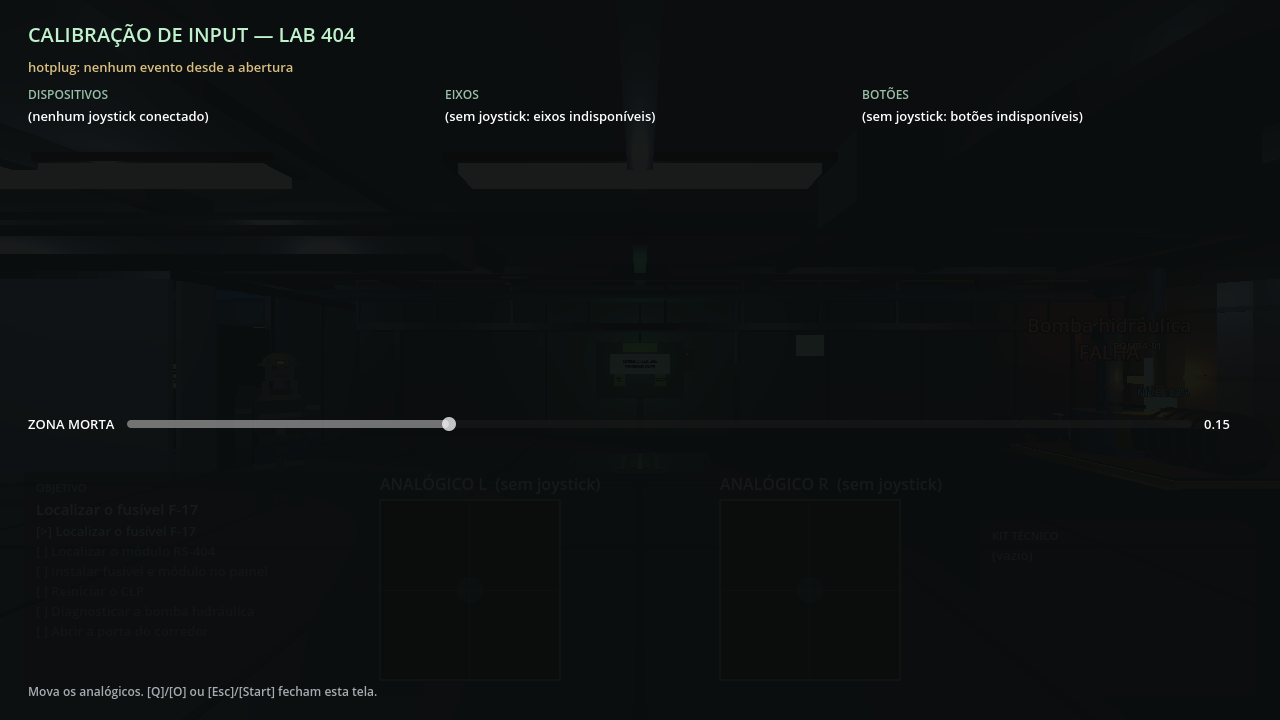
\includegraphics[width=0.86\textwidth]{input_test.png}
\caption{Tela de diagnóstico de entrada em execução: dispositivos detectados, eixos com valores instantâneos, botões pressionados, zona morta configurável e mensagem de estado da conexão.}
\label{fig:input_test}
\par\vspace{2pt}{\footnotesize Fonte: captura do autor (2026), gerada pela cena de captura do projeto em 1280$\times$720.}
\end{figure}

A tela cumpre dois papéis no projeto. O primeiro é de engenharia: como o
adaptador USB de controle (modelo de PlayStation~1) enumera botões e eixos de
maneira imprevisível, a calibração precisa ser observável --- e é essa tela
que permite descobrir, em segundos, qual índice físico corresponde a cada
ação, sem depender de tentativa e erro no jogo. O segundo papel é de
auditoria: a tela é a única parte do projeto autorizada a ler índices
numéricos de botão e eixo; todo o \emph{gameplay} consome apenas ações
semânticas, e essa separação é verificável no código.


\end{document}
